\documentclass{article}

\usepackage[preprint]{neurips_2026}

\usepackage[utf8]{inputenc}
\usepackage[T1]{fontenc}
\usepackage{hyperref}
\usepackage{url}
\usepackage{booktabs}
\usepackage{amsfonts}
\usepackage{amsmath}
\usepackage{amssymb}
\usepackage{amsthm}
\usepackage{nicefrac}
\usepackage{microtype}
\usepackage{xcolor}
\usepackage{graphicx}
\usepackage{algorithm}
\usepackage{algorithmic}
\usepackage{enumitem}
\usepackage{listings}
\usepackage{float}

\newtheorem{theorem}{Theorem}
\newtheorem{proposition}[theorem]{Proposition}
\newtheorem{lemma}[theorem]{Lemma}
\newtheorem{corollary}[theorem]{Corollary}

\theoremstyle{definition}
\newtheorem{definition}[theorem]{Definition}

\theoremstyle{remark}
\newtheorem{remark}[theorem]{Remark}

\DeclareMathOperator{\tr}{tr}
\DeclareMathOperator{\sgn}{sgn}
\DeclareMathOperator{\im}{Im}
\newcommand{\R}{\mathbb{R}}
\newcommand{\C}{\mathbb{C}}
\newcommand{\SO}{\mathrm{SO}}
\newcommand{\OG}{\mathrm{O}}
\newcommand{\SH}{Y}
\newcommand{\CG}[6]{C^{#5,\,#6}_{#1,\,#2;\,#3,\,#4}}
\newcommand{\abs}[1]{\lvert #1 \rvert}
\newcommand{\norm}[1]{\lVert #1 \rVert}
\newcommand{\conj}[1]{\overline{#1}}
\newcommand{\ip}[2]{\langle #1,\, #2 \rangle}

\theoremstyle{definition}
\newtheorem{assumption}[theorem]{Assumption}
\newtheorem{hypothesis}[theorem]{Hypothesis}


\lstset{
  language=Python,
  basicstyle=\ttfamily\small,
  keywordstyle=\bfseries,
  commentstyle=\color{gray},
  stringstyle=\color{black!60},
  frame=single,
  breaklines=true,
  columns=fullflexible,
}

\setlist[itemize]{noitemsep,topsep=2pt,partopsep=0pt}
\setlist[enumerate]{noitemsep,topsep=2pt,partopsep=0pt}
\setlength{\textfloatsep}{6pt plus 1pt minus 2pt}
\setlength{\intextsep}{6pt plus 1pt minus 2pt}
\setlength{\abovecaptionskip}{4pt}
\setlength{\belowcaptionskip}{2pt}

\title{\texttt{bispectrum}: Selective $G$-Bispectra Made Practical}

% Put this in the preamble, before \author
\newcommand{\authorblock}[4]{%
  \begin{minipage}[t]{0.43\textwidth}
    \vspace{0pt}
    \centering
    \textbf{#1}\\
    #2\\
    #3\\
    \texttt{#4}
  \end{minipage}%
}

\author{%
\normalfont
\begin{tabular*}{\textwidth}{@{\extracolsep{\fill}}cc@{}}
  \authorblock
    {Johan Mathe}
    {Atmo, Inc.}
    {San Francisco, CA}
    {johan@atmo.ai}
  &
  \authorblock
    {Adele Myers Lantow}
    {UC Santa Barbara}
    {Santa Barbara, CA}
    {adele@ucsb.edu}
  \\[5em]
  \authorblock
    {Simon Mataigne}
    {UCLouvain}
    {Louvain-la-Neuve, Belgium}
    {simon.mataigne@uclouvain.be}
  &
  \authorblock
    {Nina Miolane}
    {UC Santa Barbara}
    {Santa Barbara, CA}
    {nmiolane@ucsb.edu}
\end{tabular*}%
}

\begin{document}

\maketitle

\begin{abstract}
Many machine learning tasks are invariant under the action of a group $G$ of transformations: signal classification
can be invariant under translations, image
classification under 2D rotations, and spherical-image classification under 3D rotations. The $G$-bispectrum is a principled \emph{complete} invariant of a signal (retaining all all signal's information up to the group action) with proven benefits in machine learning and as a pooling layer in deep networks. However, its
deployment has been hampered by high computational cost and a patchwork of
group-specific implementations.
We present \texttt{bispectrum}, an open-source, fully unit-tested
PyTorch library that implements \emph{selective} $G$-bispectra for seven different group actions, as differentiable modules that can be directly incorporated into machine learning pipelines and deep learning architectures. For finite groups $G$, selectivity
reduces the computational cost from $O(|G|^2)$ to $O(|G|)$. For planar rotations, we leverage the disk bispectrum. For spherical 3D rotations,
we introduce an augmented selective bispectrum at band-limit
$L$ which reduces the cost from $O(L^3)$ to $\Theta(L^2)$ coefficients.
We profile the entire library (for which we implemented various compute optimizations), showing that it delivers near-exact $G$-invariance with its selective $G$-bispectra computed in sub-millisecond time on GPU (up to commonly used bandlimits). We evaluate the benefits of incorporating $G$-bispectra as pooling layers into deep learning architectures on three classical benchmark datasets --comparing against norm pooling,
gated pooling, Fourier-ELU pooling, max pooling, and (non-equivariant)
data-augmented convolutional baselines. Results show that $G$-bispectra consistently outperform alternatives
in the low-data, moderate-capacity regime.
Code is available at
\url{https://github.com/geometric-intelligence/bispectrum/}.
\end{abstract}
\section{Introduction}
\label{sec:intro}

Many machine learning tasks are invariant under the action of a group $G$ of transformations: signal classification
can be invariant under translations, image
classification under 2D rotations, and spherical-image classification under 3D rotations. Equivariant neural networks~\citep{cohen2016group, weiler2019general} enforce invariance by adding an invariant pooling layer to their equivariant feature maps.
Existing choices (norm pooling, gate-based pooling, max/sum
aggregation~\citep{weiler2019general}) are simple but
\emph{incomplete}: they discard information that a complete
group-invariant representation would preserve. For instance, norm pooling retains only the power spectrum of the feature map, so two signals that share the same per-frequency magnitudes but differ in their relative phases (and are therefore not related by any group element) are mapped to the same invariant descriptor.

The $G$-bispectrum is a principled
alternative~\citep{giannakis1989bispectrum, kakarala2012bispectrum,
sanborn2023bispectral, mataigne2024selective, myers2025selective}. The $G$-bispectrum is a complex-valued descriptor of a signal that is invariant under the action of a group $G$. It has three properties that make it particularly suited to learning on structured data: (i)~\textit{completeness} --- it preserves all signal
information up to the group action; (ii)~\textit{inversion} --- the signal can be
recovered from the invariant up to a group action; and
(iii)~\textit{selectivity} --- a small subset of the $G$-bispectrum's entries suffices for completeness on generic signals, a fact first observed for translations by~\citet{giannakis1989bispectrum} and recently extended to finite groups and the disk~\citep{mataigne2024selective,myers2025selective}.

\paragraph{Existing constructions of $G$-bispectra are scattered across theoretical papers and group-specific implementations.} The selective $G$-bispectrum
of~\citet{mataigne2024selective} covers signals defined over finite groups. The selective disk bispectrum from
\citet{myers2025selective} proposes a bispectrum for 2D images defined over the disk, with invariance with respect to planar rotations. The spherical bispectrum of \citet{kakarala2012bispectrum} provides a representation of spherical images that is invariant to 3D rotations; however, neither an implementation nor an empirical evaluation within machine learning pipelines has been reported to date. The classical translation bispectrum~\citep{giannakis1989bispectrum} is well-known in signal processing but likewise lacks an open, GPU-ready implementation. \citet{sanborn2023bispectral} provides a bispectral neural network implementation for cyclic groups, but it does not extend to continuous groups or general finite groups. The absence of a unified, efficient, and differentiable implementation across group actions has limited the bispectrum's adoption as a practical building block in modern deep learning pipelines.

\paragraph{Contributions.} We present, profile, and evaluate \texttt{bispectrum}, an open-source, fully unit-tested
PyTorch library that implements \emph{selective} $G$-bispectra as differentiable modules that can be directly incorporated into machine learning pipelines and deep learning architectures. Our contributions are:
\begin{enumerate}[leftmargin=*]
  \item \textbf{Software: Pytorch Library.} We implement selective
    $G$-bispectra for \emph{seven group actions} as drop-in differentiable modules with a
    uniform API unlocking practical deployment across machine learning and deep learning pipelines. We provide an efficient implementation with sub-millisecond GPU forward passes  and a fully unit-tested codebase (96 \% line coverage).
  \item \textbf{Theory: Selective Bispectrum for Spherical Rotations}
    We introduce the first selective bispectrum for 3D rotations acting on spherical images, at bandlimit $L$, reducing the cost from $O(L^3)$ to $O(L^2)$ and empirically demonstrate its completeness when augmented with a few power coefficients.
 \item \textbf{Experiments: Unified Evaluation.} We evaluate bispectral
  pooling on three classification tasks spanning planar, volumetric, and
  spherical domains, each equipped with a different symmetry group. We
  compare against norm pooling, gated pooling, Fourier-ELU pooling, max
  pooling, and data-augmented convolutional baselines. Bispectral pooling delivers
  near-exact $G$-invariance and a consistent data-efficiency
  advantage over incomplete alternatives in the low-data,
  moderate-capacity regime, converging to them at high capacity.
\end{enumerate}

Together, these contributions close the gap between the theoretical appeal of $G$-bispectra and their practical use in modern machine learning and deep learning pipelines.

\section{Mathematical Background}
\label{sec:background}

We introduce the main mathematical concepts used to define $G$-bispectra.
Given a group $G$, a \emph{representation} $\rho$ assigns each $g\in G$ a
unitary matrix $\rho(g)$ with $\rho(gh)=\rho(g)\rho(h)$; an
\emph{irreducible representation} (\emph{irrep}) has no nontrivial
invariant subspace, and the \emph{dual} $\hat{G}$ is the set of equivalence
classes of irreps. A $G$-action on a domain $X$,
$(g,x)\mapsto g\cdot x$, induces an action on signals
$(f\circ g)(x):= f(g\cdot x)$; two signals are in the same \emph{orbit}
if and only if they are related by some $g\in G$, and an \emph{invariant}
is a function constant on each orbit.
A neural network layer $\Phi$ is \emph{$G$-equivariant} if
$\Phi(\pi_{\mathrm{in}}(g)\, f) = \pi_{\mathrm{out}}(g)\, \Phi(f)$
for all $g \in G$~\citep{cohen2016group, weiler2019general}.
Stacking equivariant layers preserves equivariance, but any task requiring
a prediction independent of the group action must eventually map equivariant
features to invariant ones.

\paragraph{Bispectrum on finite groups.}
The $G$-bispectrum~\citep{kakarala1992triple, mataigne2024selective}
provides a complete invariant pooling mechanism for signals on finite
groups. Given a signal $\Theta : G \to \R$ on a finite group $G$ with
unitary irreps $\{\rho_i\}_{i\in\hat{G}}$, the \emph{$G$-Fourier
transform}~\citep{diaconis1990fourier} is
\begin{equation}\label{eq:fourier-finite}
  \mathcal{F}(\Theta)_{\rho_i}
  := \sum_{g \in G} \Theta(g)\, \rho_i(g)^{\dagger}
  \;\in\; \C^{d_i \times d_i},
\end{equation}
where $d_i = \dim(\rho_i)$. The \emph{full $G$-bispectrum} is
\begin{equation}\label{eq:bispectrum-def}
  \beta(\Theta)_{\rho_1,\rho_2}
  = \bigl[\mathcal{F}(\Theta)_{\rho_1} \otimes
    \mathcal{F}(\Theta)_{\rho_2}\bigr]\,
    C_{\rho_1,\rho_2}\,
    \Bigl[\bigoplus_{\rho \in \rho_1 \otimes \rho_2}
      \mathcal{F}(\Theta)_{\rho}^{\dagger}\Bigr]\,
    C_{\rho_1,\rho_2}^{\dagger},
\end{equation}
where $C_{\rho_1,\rho_2}$ is the unitary Clebsch--Gordan matrix that
block-diagonalizes the tensor product $\rho_1 \otimes \rho_2$ into
irreducible summands. Each matrix
$\beta(\Theta)_{\rho_1,\rho_2}$ is $G$-invariant, and the full collection
$\{\beta(\Theta)_{\rho_1,\rho_2}\}_{(\rho_1,\rho_2)\in\hat{G}^2}$
is a complete $G$-invariant for generic signals (i.e.\ those with
nonsingular Fourier coefficients)~\citep{kakarala1992triple}.
The full bispectrum has $O(|G|^2)$ scalar entries.
\citet{mataigne2024selective} shows that a breadth-first search over
the Kronecker product table of $\hat{G}$ selects $O(|G|)$ bispectral
coefficients that remain complete; for example, the octahedral group
drops from $576$ to $172$ scalars.

\paragraph{Bispectrum on the disk.}
The disk bispectrum~\citep{zhao2014rotationally, myers2025selective}
is an $\SO(2)$-invariant descriptor for planar images defined on the
unit disk $\mathbb{D}$. A signal $f : \mathbb{D} \to \R$ is expanded in
disk harmonics (eigenfunctions of the Laplacian on $\mathbb{D}$):
\begin{equation}\label{eq:disk-harmonics}
  \psi_{nk}(r,\theta) = c_{nk}\, J_n(\lambda_{nk}\, r)\, e^{in\theta},
\end{equation}
where $J_n$ is the Bessel function of order $n$, $\lambda_{nk}$ its
$k$-th positive root, and $c_{nk}$ a normalization constant.
The disk harmonic (DH) coefficients $a_{n,k}$ are equivariant to planar
rotations: if $f' = f \circ R_\phi$ then
$a^{f'}_{n,k} = e^{in\phi}\, a^{f}_{n,k}$.
For a bandlimit yielding $m$ coefficients with maximum angular frequency
$N_m$, the \emph{full disk bispectrum}~\citep{zhao2014rotationally} is
\begin{equation}\label{eq:bispectrum-disk}
  b_{j_1,j_2,k_3}
  = a_{n_{j_1},k_{j_1}}\, a_{n_{j_2},k_{j_2}}\,
    a_{n_{j_1}+n_{j_2},\,k_3}^{*},
\end{equation}
with $O(m^3 / N_m)$ coefficients. \citet{myers2025selective} introduces
the \emph{selective disk bispectrum}, restricting to two families of
triples that yield $O(m)$ coefficients while remaining a complete
$\SO(2)$-invariant (under the genericity condition $a_{n,1}\neq 0$ for
all angular orders $n$).

\paragraph{Bispectrum on the sphere.}
The spherical bispectrum~\citep{kakarala2012bispectrum} is an
$\SO(3)$-invariant descriptor for band-limited signals on $S^2$.
A real signal $f : S^2 \to \R$ at band limit $L$ has spherical harmonic
coefficients $a_\ell^m$ with coefficient vectors
$\mathbf{F}_\ell = (a_\ell^{-\ell},\ldots,a_\ell^{\ell})^\top
\in \C^{2\ell+1}$, transforming under $g\in\SO(3)$ as
$\mathbf{F}_\ell \mapsto D^\ell(g)\,\mathbf{F}_\ell$, where $D^\ell$
is the $(2\ell{+}1)$-dimensional Wigner $D$-matrix.
For each admissible triple $(\ell_1,\ell_2,\ell)$ satisfying the
triangle inequality
$|\ell_1 - \ell_2| \le \ell \le \ell_1 + \ell_2$, the
\emph{bispectral coefficient} is
\begin{equation}\label{eq:bispectrum-sphere}
  \beta_{\ell_1,\ell_2,\ell}
  = \sum_{\substack{m_1,\,m_2,\,m \\ m_1+m_2=m}}
    \CG{\ell_1}{m_1}{\ell_2}{m_2}{\ell}{m}\;
    a_{\ell_1}^{m_1}\,a_{\ell_2}^{m_2}\,\conj{a_\ell^m},
\end{equation}
where $\CG{\ell_1}{m_1}{\ell_2}{m_2}{\ell}{m}$ denotes the
Clebsch--Gordan coefficient
$\langle \ell_1, m_1;\, \ell_2, m_2 \mid \ell, m \rangle$.
The full set has $\Theta(L^3)$ scalars. On homogeneous spaces such as
$S^2$, the Fourier coefficients are rank-deficient (vectors rather than
full-rank matrices), so the operator-bispectrum completeness
of~\citet{kakarala2012bispectrum} does not directly
apply~\citep{kondor2007novel}. In Section~\ref{sec:so3-selective} we
introduce a selective construction that reduces the scalar bispectrum to
$\Theta(L^2)$ entries and empirically demonstrate its completeness via
signal reconstruction.

Throughout this paper, we use the term \emph{$G$-bispectrum} to refer
collectively to the bispectra defined by
Equations~\eqref{eq:bispectrum-def},~\eqref{eq:bispectrum-disk},
and~\eqref{eq:bispectrum-sphere} for the simplicity of terminology.




\section{Related Work}
\label{sec:related}
This section reviews related work along three axes: (i) equivariant and invariant libraries that provide building blocks for $G$-invariant architectures, (ii) bispectral methods in neural networks and their computational trade-offs, and (iii) alternative invariant constructions (CG products, scattering) that compete with or complement the $G$-bispectrum. 

\paragraph{Equivariant network libraries.}
The \texttt{escnn}~\citep{cesa2022program} and \texttt{e3nn}~\citep{geiger2022e3nn}
libraries provide general-purpose equivariant convolution layers for 2D and 3D
groups respectively, and \texttt{lie-nn}~\citep{batatia2023general}
provides general Lie-group representation primitives (irreducible
representations, Clebsch--Gordan decompositions, tensor products) on
top of which custom equivariant layers can be built. These libraries
implement equivariant \emph{feature maps} but leave the choice of
invariant pooling to the user (typically norm or gate). Our library is
complementary: it provides the invariant map as a drop-in
\texttt{nn.Module} that plugs into architectures built with any of these
frameworks.

\paragraph{Bispectral approaches in neural networks.}
\citet{sanborn2023bispectral} introduced bispectral neural networks (BNNs),
using the full $G$-bispectrum as an invariant nonlinearity for $C_n$ and $D_n$.
\citet{oreiller2022bispectral} applied bispectral CNNs to medical imaging
with a fixed set of hand-selected triples. Both use the full (quadratic-cost)
bispectrum and provide implementations tied to specific architectures.
Our library generalizes to seven group/domain pairs, defaults to the
$O(|G|)$ selective reduction~\citep{mataigne2024selective}, and exposes
a framework-agnostic API.
\citet{chevalley2024bispectral} explores bispectral signatures for data
characterization, using bispectra as descriptors rather than learnable
pooling primitives.
Outside the equivariant-network setting,
\texttt{PyBispectra}~\citep{binns2025pybispectra} computes bispectrum
and bicoherence statistics of one-dimensional time-series signals for
electrophysiology applications such as phase-amplitude coupling and
time-delay estimation; the underlying 1D bispectrum is translation-invariant
by construction, but the toolbox is not designed as a neural-network
pooling layer.

\paragraph{Bispectra on homogeneous and non-homogeneous spaces.}
The selective $G$-bispectrum
construction~\citep{mataigne2024selective} reduces the cost of the
$G$-bispectrum from $O(|G|^2)$ to $O(|G|)$ scalars on finite groups.
\citet{myers2025selective} extends the selective construction to the
disk, where $\SO(2)$ acts on a non-homogeneous space.
\citet{kakarala2012bispectrum} treats the $\SO(3)$-on-$\SO(3)$
bispectrum and the closely related sphere case via Wigner-$D$ irreps.
The matrix (vector) bispectrum on $S^2$ is the homogeneous-space form
on which our scalar contractions and CG power augmentation are built.

\paragraph{Invariant theory and scattering.}
The wavelet scattering transform~\citep{mallat2012scattering} provides
translation-invariant representations via iterated modulus operations;
\citet{esteves2018spherical} extends this to the sphere. Unlike the
$G$-bispectrum, scattering representations are stable but generally
incomplete; they discard inter-scale phase information.
The $G$-bispectrum's completeness
guarantee~\citep{giannakis1989bispectrum, kakarala2012bispectrum} is
its distinguishing theoretical advantage.

\begin{table}[t]
  \caption{Trade-offs among invariant nonlinearities. The selective
    bispectrum (this work) is the only exact, complete, linear-cost
    option for finite groups; our $\SO(3)$-on-$S^2$ variant achieves
    $\Theta(L^2)$ with empirical completeness
    (Sec.~\ref{sec:so3-selective}).
    $^\dagger$Genericity: completeness holds outside a measure-zero
    algebraic subvariety.}
  \label{tab:nonlinearity-comparison}
  \centering
  \small
  \setlength{\tabcolsep}{4pt}
  \begin{tabular}{lcccl}
    \toprule
    Nonlinearity & Complete? & Coefficients & Forward cost & Key limitation \\
    \midrule
    Norm              & No              & $O(|G|)$   & $O(|G|)$          & Discards phase \\
    Gate              & No              & $O(|G|)$   & $O(|G|)$          & Scalar bottleneck \\
    Fourier pointwise & Yes$^\ddagger$  & $O(|G|)$   & $O(|G| \log |G|)$ & Aliasing \\
    Full bispectrum (finite $G$)      & Yes & $O(|G|^2)$   & $O(|G|^3)$ & Quadratic cost \\
    Full bispectrum ($\SO(3)$/$S^2$)  & Yes & $\Theta(L^3)$ & $O(L^4)$  & Cubic cost \\
    \midrule
    Selective bispectrum (finite $G$) & Yes       & $O(|G|)$      & $O(|G|^2)$ & Genericity assumption$^\dagger$ \\
    Augmented selective $\SO(3)$/$S^2$ (ours) & Empirical & $\Theta(L^2)$ & $O(L^3)$   & Proof of concept only \\
    \bottomrule
  \end{tabular}

  \vspace{0.3em}
  {\small $^\ddagger$Complete pre-aliasing; the pointwise nonlinearity introduces aliasing that may break completeness in practice.}
\end{table}

Table~\ref{tab:nonlinearity-comparison} summarizes the trade-offs between
exactness, completeness, and computational cost across existing invariant
pooling layers. Norm pooling and gated nonlinearities are exact
invariants but \emph{incomplete}. Fourier-space pointwise
nonlinearities preserve completeness but sacrifice exactness through
\mbox{aliasing~\citep{weiler2019general}}. The full bispectrum is exact and
complete but costs $O(|G|^2)$ coefficients. The \emph{selective}
bispectrum (introduced below) preserves both exactness and completeness
while using only $O(|G|)$ coefficients on generic signals.


\section{The \texttt{bispectrum} Library}
\label{sec:library}

\paragraph{Design and implementation.} \label{sec:design} Every $G$/domain pair is a \texttt{torch.nn.Module} named
\texttt{\{Group\}on\{Domain\}} (e.g.\ \texttt{SO3onS2});
Table~\ref{tab:supported-groups} lists all seven modules. Each exposes a
uniform API: \texttt{forward(f)} returns the selective invariants,
\texttt{fourier(f)} the group Fourier coefficients, and
\texttt{invert(beta)} the reconstructed signal up to group-action
indeterminacy (where available). Modules default to $O(|G|)$
selective coefficients (\texttt{selective=False} restores the full
$O(|G|^2)$ set), precompute CG matrices / DFT kernels / Bessel
roots as non-learnable buffers, and depend only on
PyTorch~\citep{paszke2019pytorch}, NumPy~\citep{harris2020numpy},
and \texttt{torch\_harmonics}~\citep{bonev2023spherical} (for
\texttt{SO3onS2}). Test suite line coverage is 96.8\%; a minimal
usage example is in Appendix~\ref{app:api-example}.

\begin{table}[tbp]
  \caption{Seven group/domain pairs in the \texttt{bispectrum} library,
    each a drop-in \texttt{nn.Module} with uniform API.
    \texttt{SO2onS1} is the continuous-$n$ limit of \texttt{CnonCn}.}
  \label{tab:supported-groups}
  \centering
  \small
  \begin{tabular*}{\linewidth}{@{\extracolsep{\fill}}llll@{}}
    \toprule
    Module & Group / Domain & Output mode & Reference \\
    \midrule
    \texttt{CnonCn} & $C_n$ on $C_n$ & selective + full & \citep{sanborn2023bispectral} \\
    \texttt{SO2onS1} & $\SO(2)$ on $S^1$ & selective + full & \citep{mataigne2024selective} \\
    \texttt{TorusDnTorus} & $\mathbb{T}^d$ & selective + full & \citep{mataigne2024selective} \\
    \texttt{DnonDn} & $D_n$ on $D_n$ & selective & \citep{mataigne2024selective} \\
    \texttt{SO2onDisk} & $\SO(2)$ on disk & selective & \citep{myers2025selective} \\
    \texttt{SO3onS2} & $\SO(3)$ on $S^2$ & selective + full & \citep{kakarala2012bispectrum}, this paper \\
    \texttt{OctaonOcta} & chiral octahedral $O$ & selective & \citep{mataigne2024selective} \\
    \bottomrule
  \end{tabular*}
\end{table}



\paragraph{Profiling.} \label{sec:benchmarks} We profile the library on a single NVIDIA H100 80\,GB GPU
(PyTorch 2.10, batch\,=\,16 for the forward pass and 4 for inversion,
median wall-clock via \texttt{torch.utils.benchmark}); results are in
Table~\ref{tab:benchmarks}.
The selective forward pass is sub-millisecond for all six modules:
finite abelian groups ($C_n$: 0.14\,ms, $\mathbb{T}^2$: 0.07\,ms),
$D_n$ (0.54\,ms), $\mathrm{SO}(2)$ on the disk (0.22\,ms),
$\mathrm{SO}(3)$ on $S^2$ at $L{=}16$ (0.48\,ms), and the octahedral
group (0.68\,ms), making it negligible relative to backbone computation.
GPU throughput scales linearly with batch size, exceeding
$10^7$~samples/s for $C_n$ and $\mathbb{T}^2$
(Appendix~\ref{app:bench}). Six modules are presented; the seventh,
\texttt{SO2onS1}, subclasses \texttt{CnonCn} with $n = L{+}1$ and has
identical runtime to the corresponding \texttt{CnonCn} row at matched
$|G|$. Coefficient-count scaling and additional plots are in
Appendix~\ref{app:bench} (Figure~\ref{fig:coeff-scaling}).

\begin{table}[tbp]
  \centering
  \caption{Selective forward pass is sub-millisecond for all modules;
    selectivity reduces coefficients by up to $512\times$.
    Median wall-clock, NVIDIA H100, batch\,=\,16.
    ``--'': not implemented.}
  \label{tab:benchmarks}
  \small
  \setlength{\tabcolsep}{3.5pt}
  \begin{tabular*}{\linewidth}{@{\extracolsep{\fill}}llrrrrr@{}}
    \toprule
    Module & $G$ & $|G|/L$ & \multicolumn{2}{c}{Coefs} & \multicolumn{2}{c}{Fwd (ms)} \\
    \cmidrule(lr){4-5} \cmidrule(lr){6-7}
     & & & Sel. & Full & Sel. & Full \\
    \midrule
    \texttt{CnonCn} & $C_{128}$ & 128 & 128 & 8{,}256 & 0.14 & 8.90 \\
    \texttt{TorusOnTorus} & $C_{32}{\times}C_{32}$ & 1{,}024 & 1{,}024 & 524{,}800 & 0.07 & 0.31 \\
    \texttt{DnonDn} & $D_{32}$ & 64 & 245 & -- & 0.54 & -- \\
    \texttt{SO2onDisk} & $\mathrm{SO}(2)$ & $L{=}16$ & 105 & -- & 0.22 & -- \\
    \texttt{SO3onS2} & $\mathrm{SO}(3)$ & $L{=}16$ & 430 & -- & 0.48 & -- \\
    \texttt{OctaonOcta} & $O$ & 24 & 172 & -- & 0.68 & -- \\
    \bottomrule
  \end{tabular*}
\end{table}



\section{Augmented selective $\SO(3)$ invariant on $S^2$}
\label{sec:so3-selective}

This section instantiates the $G$-bispectrum framework of
Section~\ref{sec:background} on $S^2$ and is the main theoretical
contribution: we construct $\Phi_{\mathrm{sel}}$, an
$\SO(3)$-invariant of size $\Theta(L^2)$ on band-limited spherical
signals, and probe its completeness empirically.

\paragraph{Setup and construction.} A real signal $f : S^2 \to \R$
band-limited at degree~$L$ is determined by its spherical harmonic
coefficients $a_\ell^m\in\C$, $m=-\ell,\dots,\ell$, $\ell=0,\dots,L$,
gathered into vectors $\mathbf{F}_\ell = (a_\ell^{-\ell},\dots,
a_\ell^{\ell})^\top \in \C^{2\ell+1}$ that transform as
$\mathbf{F}_\ell \mapsto D^\ell(g)\,\mathbf{F}_\ell$ under
$g\in\SO(3)$ ($D^\ell$ the Wigner-$D$ matrix); the reality condition
leaves $(L{+}1)^2$ real degrees of freedom
(Appendix~\ref{sec:app-setup}).
A triple $(\ell_1,\ell_2,\ell)$ is \emph{CG-admissible} if it
satisfies the triangle inequality
$|\ell_1-\ell_2|\le\ell\le\ell_1+\ell_2$. The scalar bispectral
coefficient at such a triple is
\begin{equation}\label{eq:s6-bispectrum}
  \beta_{\ell_1,\ell_2,\ell}
  = \!\!\!\sum_{\substack{m_1,m_2,m\\ m_1+m_2=m}}\!\!\!
    \CG{\ell_1}{m_1}{\ell_2}{m_2}{\ell}{m}\,
    a_{\ell_1}^{m_1}\,a_{\ell_2}^{m_2}\,\conj{a_\ell^m},
\end{equation}
where $\CG{\ell_1}{m_1}{\ell_2}{m_2}{\ell}{m}$ is the Clebsch--Gordan
coefficient. The full set has $\Theta(L^3)$ scalars. The orbit space
$\R^{(L+1)^2}/\SO(3)$ has dimension $(L{+}1)^2 - 3$; by a rank
argument, any smooth complete $\SO(3)$-invariant must therefore have
at least $\Omega(L^2)$ live components
(Proposition~\ref{prop:app-lower-bound}). 

\paragraph{The augmented selective invariant.} We define
$\Phi_{\mathrm{sel}}(f)$ as the output of
Algorithm~\ref{alg:so3-augmented}
(Appendix~\ref{sec:app-selective-index}). Its index set is built
degree-by-degree. At low degrees $\ell\le L_{\mathrm{seed}}:=\min(L,4)$,
the \emph{seed} $\mathcal{S}_{\mathrm{seed}}$ collects every
CG-admissible triple that is non-vanishing on real signals (a
constant-size block: $24$ entries at $L_{\mathrm{seed}}=4$). For each
higher degree $\ell > L_{\mathrm{seed}}$, the algorithm appends a
\emph{bootstrap block} $\mathcal{T}_\ell$ of $2\ell{+}1$ scalar
bispectral entries linear in the new coefficients $\mathbf{F}_\ell$;
the self-couplings $\beta_{\ell,\ell,\ell'}$ for
$\ell'\in\{2,4,\dots\}$, $\ell'\le\ell$ (restricted to even $\ell'$
because odd $\ell'$ produces a repeated-index, odd-parity entry that
vanishes identically on real signals;  Proposition~\ref{prop:app-odd-vanishing}) and a greedily-chosen set
of CG-power scalars
$P_{\ell_1,\ell_2,\ell} := \lVert(\mathbf{F}_{\ell_1}\otimes
\mathbf{F}_{\ell_2})|_\ell\rVert^2$, added until the per-degree
Jacobian of $\Phi_{\mathrm{sel}}|_\ell$ has full rank.
Because $\Phi_{\mathrm{sel}}$ mixes degree-$3$ bispectrum entries
with degree-$4$ CG-power scalars, we call it an \emph{augmented
selective invariant} rather than a bispectrum; the term
``selective bispectrum'' refers strictly to its bispectral component
$\mathcal{S}_\beta$. The total size is
$|\Phi_{\mathrm{sel}}| = \Theta(L^2)$
(Proposition~\ref{prop:app-output-size}); concretely, at $L=15$
(resp.\ $L=16$) it produces $384$ (resp.\ $430$) real scalars vs.\
$2{,}056$ admissible triples in the full bispectrum at $L=15$
(Table~\ref{tab:app-counts}). Algorithm~\ref{alg:selective-bsp-so3}
below summarises the bispectral-triple selection; the full index
set, with even self-couplings and CG-power augmentation, is
Algorithm~\ref{alg:so3-augmented} in
Appendix~\ref{sec:app-selective-index}.

\begin{algorithm}[H]
\caption{Bispectral triples in the Mataigne-style BFS chain
  (mirrors~\citet{mataigne2024selective}, Alg.~1): seed block at low
  degrees plus per-degree bootstrap blocks. The full index set of
  $\Phi_{\mathrm{sel}}$, including even self-couplings
  $\beta_{\ell,\ell,\ell'}$ and CG-power scalars
  $P_{\ell_1,\ell_2,\ell}$, is built by
  Algorithm~\ref{alg:so3-augmented} in
  Appendix~\ref{sec:app-selective-index}.}
\label{alg:selective-bsp-so3}
\small
\begin{algorithmic}[1]
\STATE \textbf{Input:} band-limit $L$,
  seed cutoff $L_{\mathrm{seed}} = \min(L,4)$
\STATE $\mathcal{L}_\beta \leftarrow$ all admissible triples
  $(\ell_1,\ell_2,\ell)$ with $\ell\le L_{\mathrm{seed}}$
  \COMMENT{seed block $\mathcal{S}_{\mathrm{seed}}$}
\FOR{$\ell = L_{\mathrm{seed}}{+}1, \dotsc, L$}
  \STATE append the bootstrap block $\mathcal{T}_\ell$
    to $\mathcal{L}_\beta$
    \COMMENT{$2\ell{+}1$ entries linear in $\mathbf{F}_\ell$;
      tabulated in Appendix~\ref{sec:app-selective-index}}
\ENDFOR
\RETURN $\{\beta_{\ell_1,\ell_2,\ell}(f) :
  (\ell_1,\ell_2,\ell)\in\mathcal{L}_\beta\}$
\end{algorithmic}
\end{algorithm}


\paragraph{Empirical proof of concept: bispectrum completeness.}
\label{sec:so3-recon}
Whether $\Phi_{\mathrm{sel}}$ is a \emph{complete} $\SO(3)$-invariant
---i.e., whether $\Phi_{\mathrm{sel}}(f) = \Phi_{\mathrm{sel}}(g)$
implies $f, g$ lie in the same orbit---can be probed empirically by
attempting to invert it: if $\Phi_{\mathrm{sel}}$ is complete, any
signal $\hat f$ matching $\Phi_{\mathrm{sel}}(R\cdot f)$ must agree
with $R\cdot f$ up to a global rotation, so consistent recovery of
the input is operational evidence that no orbit information is lost.
We run this test on Spherical MNIST digits band-limited at
$L = 12$.\footnote{We use $L{=}12$ here rather than the classifier's
$L{=}15$ to keep the reconstruction residual safely below the SHT
discretization floor at the $64{\times}128$ grid; protocol details
are in Appendix~\ref{app:so3-recon}.} For each source signal
$f:S^2\to\R$ we draw a uniform random rotation $R\in\SO(3)$, compute
$\Phi_{\mathrm{sel}}(R\cdot f)$, and recover $\hat f$ by gradient
descent from a random Gaussian initialization, minimizing
$\lVert \Phi_{\mathrm{sel}}(\hat f) -
\Phi_{\mathrm{sel}}(R\cdot f)\rVert^2 / \lVert
\Phi_{\mathrm{sel}}(R\cdot f)\rVert^2$ (Adam, multi-restart,
cosine-annealed LR). The residual orbit ambiguity is then removed by
Procrustes alignment over $\SO(3)$ on a quaternion parameterization,
fitting $\hat R$ to minimize $\lVert \hat R\cdot\hat f -
R\cdot f\rVert^2$.

\begin{figure}[t]
  \centering
  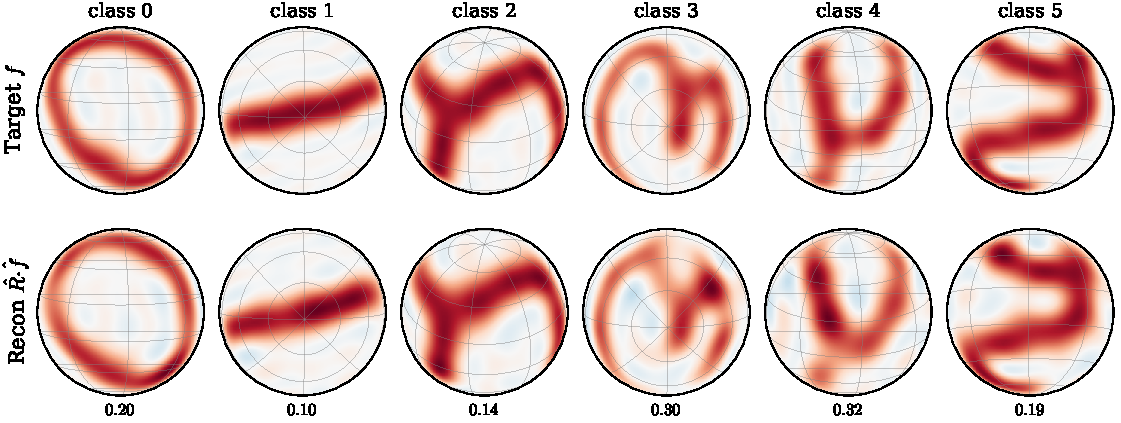
\includegraphics[width=0.9\linewidth]{experiments/spherical_mnist_reconstruction/figures/paper_orbits.pdf}
  \caption{$\Phi_{\mathrm{sel}}$ preserves enough information to
    recover signals up to rotation ($L{=}12$). Top: targets.
    Bottom: reconstructions from $\Phi_{\mathrm{sel}}$ alone,
    Procrustes-aligned. Median image residual ${\approx}0.20$;
    bispectrum residuals ${\sim}10^{-3}$.}
  \label{fig:so3-reconstruction}
\end{figure}

\paragraph{Takeaways.}
Bispectrum residuals reach
$\lVert\Delta\Phi\rVert/\lVert\Phi\rVert \sim 10^{-4}$--$10^{-3}$
(below the SHT-discretization invariance noise floor of
${\sim}8\times 10^{-3}$ at this grid); the aligned image residuals
$\lVert\hat R\cdot\hat f - f\rVert/\lVert f\rVert \sim 0.1$--$0.3$
are consistent with local optimization error or conditioning effects,
and we did not observe a systematic missing-information failure mode,
but the experiment does not rule out incompleteness or near-collisions
in feature space. Visually, $\hat R\cdot\hat f$ aligns with $f$ up to
rotation across all six digit classes shown
(Figure~\ref{fig:so3-reconstruction}; the same behaviour holds across
our 8-digit sweep, see Appendix~\ref{app:so3-recon}). We read this as
proof-of-concept evidence that $\Phi_{\mathrm{sel}}$ preserves
substantial orbit information on band-limited signals; a formal
completeness proof remains open.


\section{Experiments}
\label{sec:experiments}

We evaluate the benefits of incorporating $G$-bispectra, as implemented in the library, as pooling layers of deep learning architectures. We consider three classical benchmarks spanning discrete and continuous
groups: 2D histopathology classification under $C_8$ (Section~\ref{sec:pcam}), 3D organ classification under octahedral group
(Section~\ref{sec:organ3d}), and spherical digit
classification under $\SO(3)$ (Section~\ref{sec:smnist}).

\subsection{2D histopathology classification under cyclic symmetry}
\label{sec:pcam}

\paragraph{Setup.} We evaluate five invariant pooling strategies on
PatchCamelyon~\citep{veeling2018rotation} (PCam), which consists of 327K histopathology
patches with binary metastasis labels. All equivariant models share a
$C_8$-equivariant DenseNet~\citep{huang2017densenet} backbone following
\citet{veeling2018rotation}; they differ only in the terminal invariant map:
norm pooling, gated pooling, Fourier-ELU, and selective bispectrum via
\texttt{CnonCn}$(n{=}8)$. A standard CNN trained with
data augmentation drawn uniformly from the group $C_8$
(``\emph{augmented CNN}'') serves as the non G-equivariant baseline. We
sweep growth rates to vary capacity (30K--1.6M params) and train on
$10\%$ of the PCam training set (an image-level subsample, not a
group-orbit subsample, drawn before any group augmentation) with
AdamW~\citep{loshchilov2019adamw}. Full model descriptions are in
Appendix~\ref{app:pcam-details}.

\paragraph{Results.}
Figure~\ref{fig:pcam-pareto} shows the full Pareto sweep (AUC vs.\
parameter count, ranking, data efficiency); multi-seed statistics at
matched ${\sim}100$K params are in
Table~\ref{tab:pcam-results} (Appendix~\ref{app:pcam-details}).
At matched capacity (${\sim}100$K params, 10\% data), all four equivariant
pooling methods substantially outperform the standard augmented CNN
(AUC $0.896$). Fourier-ELU leads slightly ($0.945$), followed by
NormReLU ($0.942$), bispectrum and gated (both $0.941$).
At 1\% data, the bispectrum leads all methods ($0.912$), outperforming
NormReLU ($0.873$) and Fourier-ELU ($0.876$). This data-efficiency
advantage narrows as the training set grows, consistent with complete
invariants providing a stronger inductive bias when data is scarce.

\begin{figure}[tbp]
  \centering
  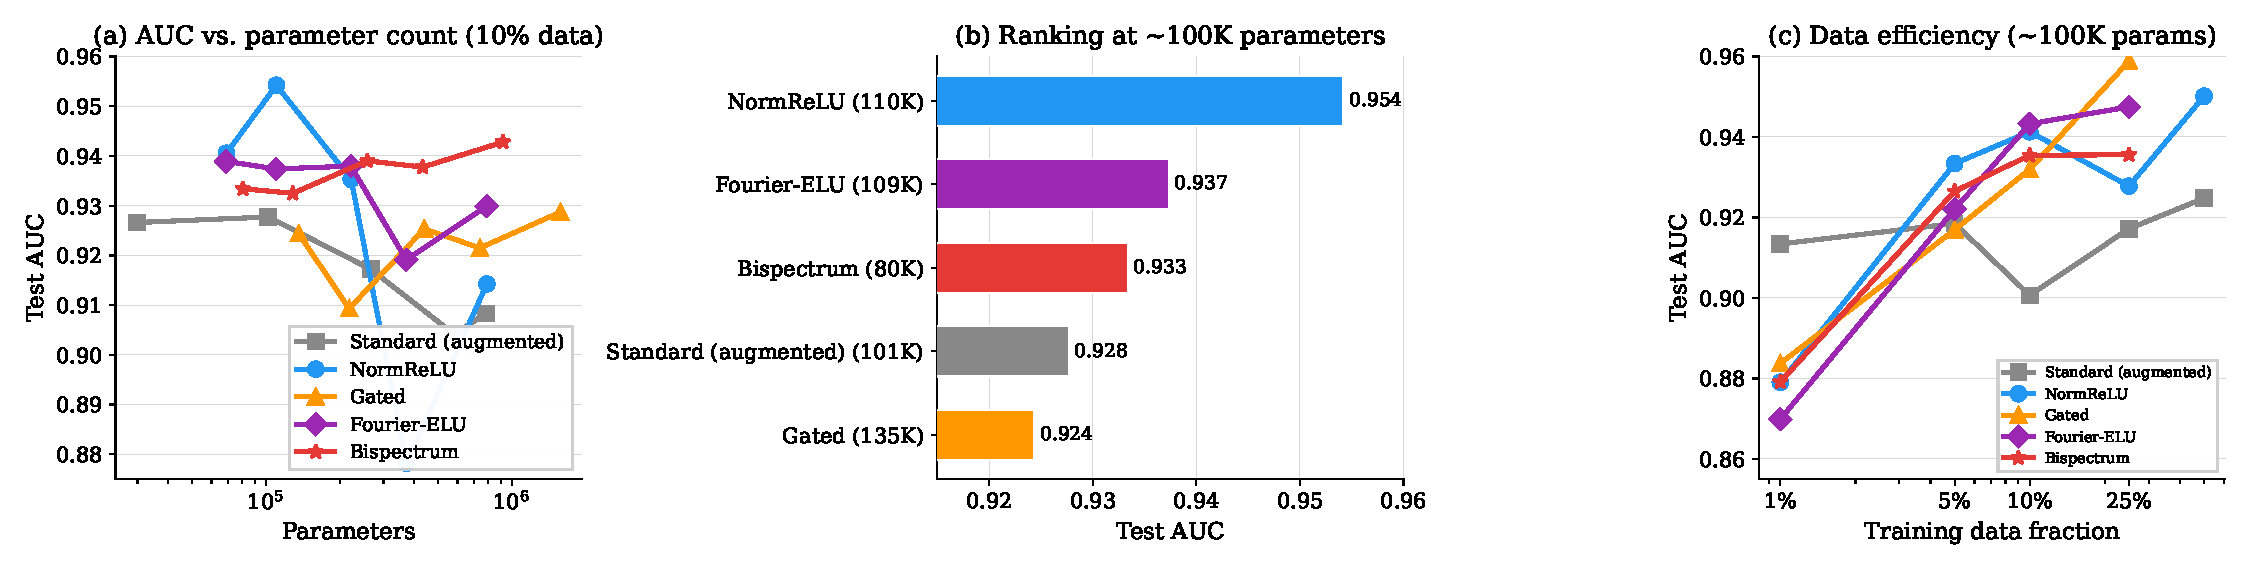
\includegraphics[width=\linewidth]{experiments/pcam/pareto_analysis.pdf}
  \caption{Bispectral pooling on PatchCamelyon ($C_8$, 10\% data).
    \textbf{(a)}~All equivariant methods dominate the augmented CNN;
    the bispectrum is most stable across capacities.
    \textbf{(b)}~At ${\sim}100$K params, methods cluster within
    $0.5$pp.
    \textbf{(c)}~At 1\% data the bispectrum leads ($0.912$ AUC),
    consistent with complete invariants compensating for scarce data.
    Multi-seed statistics in
    Table~\ref{tab:pcam-results} (Appendix~\ref{app:pcam-details}).}
  \label{fig:pcam-pareto}
\end{figure}

\subsection{3D organ classification under octahedral symmetry}
\label{sec:organ3d}

\paragraph{Setup.} To evaluate the \texttt{OctaonOcta} module for the chiral octahedral group
$O$ ($|O|=24$), we design a controlled 3D experiment on
OrganMNIST3D~\citep{medmnistv2} (1{,}742 abdominal CT volumes, $28^3$
voxels, 11 classes). All equivariant variants share an $O$-equivariant 3D
ResNet backbone with exact voxel-permutation kernels. We compare four models: a translation-equivariant standard 3D CNN trained with
octahedral data augmentation (the ``\emph{augmented CNN}'' baseline,
16K params); the $O$-equivariant ResNet with terminal norm pool
(375K params); with terminal max pool (374K params); and with terminal
selective bispectrum via \texttt{OctaonOcta} (463K, 172 invariant
scalars). Models are trained with AdamW~\citep{loshchilov2019adamw} for
100 epochs with three seeds; rotation robustness is measured over all
24 octahedral rotations of the test set. Published baselines and
wider-channel experiments are in Appendix~\ref{app:organ3d-details}.
We define the \emph{rotation robustness} $\sigma_{\mathrm{rot}}$ as the standard deviation of test accuracy when the entire test set is evaluated under every group rotation (24 octahedral rotations for OrganMNIST3D; 10 random $\SO(3)$ rotations for Spherical MNIST); a truly invariant model has $\sigma_{\mathrm{rot}}=0$.

\paragraph{Results.} Table~\ref{tab:organ3d-results} (Appendix~\ref{app:organ3d-details}) and Figure~\ref{fig:data-efficiency} report the key findings. All equivariant models achieve $\sigma_{\mathrm{rot}}\le 0.0005$
while the augmented CNN drops ${\sim}2.5$\,pp under rotation. The
bispectrum ($72.6\%$) matches max pool ($73.0\%$) and substantially
outperforms norm pool ($56.8\%$) and Regular SE(3)
convolutions~\citep{kuipers2023regular} ($69.8\%$).
At reduced data (Figure~\ref{fig:data-efficiency}), the bispectrum's
advantage widens: at 5\% data it reaches $33.2\%$ vs.\ $18.9\%$ for max
pool. At higher capacity (6M params,
Appendix~\ref{app:organ3d-details}), max pool overtakes the bispectrum,
suggesting the completeness advantage is specific to the data-limited
regime.

\begin{figure}[hbp]
  \centering
  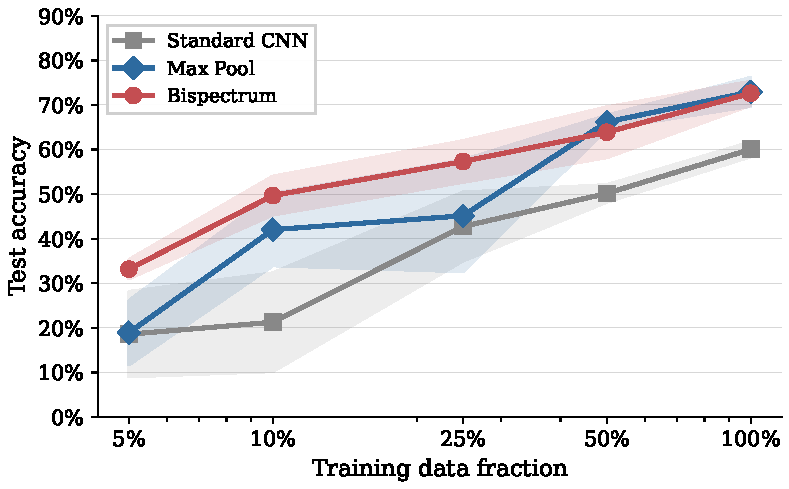
\includegraphics[width=0.78\linewidth]{experiments/organ3d/data_efficiency.pdf}
  \caption{Data efficiency on OrganMNIST3D. At 5\% data, the
    bispectrum reaches $33.2\%$ vs.\ $18.9\%$ for max pool; the gap
    narrows as data increases. Mean over 3 seeds; shaded: $\pm 1$ std.}
  \label{fig:data-efficiency}
\end{figure}

\subsection{Spherical MNIST: SO(3) invariance on the sphere}
\label{sec:smnist}

The preceding experiments validate bispectral pooling for finite groups
($C_8$ and the octahedral group $O$). To evaluate the library's continuous
group support, we test \texttt{SO3onS2}---the augmented selective
$\SO(3)$ invariant on the 2-sphere
(Section~\ref{sec:so3-selective})---on Spherical
MNIST~\citep{cohen2018spherical}, the standard benchmark for
rotation invariance on $S^2$.

\paragraph{Setup.}
MNIST digits are stereographically projected onto a
$64\times 128$ equiangular grid; we compute
$\Phi_{\mathrm{sel}}$ at $\ell_{\max}=15$ ($N=384$ live real
components, stored as 384 complex tensors by the library), apply
sign-preserving $\operatorname{sign}(x)\log(1+|x|)$ to real and
imaginary parts ($2N=768$ real channels; one channel per
bispectral entry is structurally zero by parity but we feed both
since the log transform is per-channel injective and cheap), and
feed a 3-layer MLP (232K params). Controls: a power-spectrum MLP at 11K
params (equally invariant but \emph{incomplete}, discarding
inter-harmonic phase), a matched 166K-param version isolating
capacity vs.\ completeness, and a non-invariant CNN directly on the
equirectangular image at 185K params.
Following \citet{cohen2018spherical}, we evaluate under three
protocols NR/NR, R/R, and the most challenging NR/R; each run uses
three seeds, and rotation robustness $\sigma_{\mathrm{rot}}$ is
measured over 10 random $\SO(3)$ rotations of the test set.

\begin{table}[tbp]
  \caption{Spherical MNIST (mean $\pm$ std, 3 seeds). The bispectrum
    reaches $95.0\%$ with $\sigma_{\mathrm{rot}} \sim 10^{-4}$; the
    power spectrum plateaus at ${\sim}79\%$ even at matched capacity,
    confirming incompleteness as the bottleneck. The standard CNN
    collapses to $13.8\%$ under unseen rotations (NR/R).
    Reference numbers from \citet{cohen2018spherical}.}
  \label{tab:smnist-results}
  \centering
  \small
  \setlength{\tabcolsep}{3pt}
  \begin{tabular}{lrcccc}
    \toprule
    Model & Params & NR/NR $\uparrow$ & R/R $\uparrow$ & NR/R $\uparrow$
      & $\sigma_{\mathrm{rot}}$ $\downarrow$ \\
    \midrule
    Cohen planar CNN & --- & $0.98$ & $0.23$ & $0.11$ & --- \\
    Cohen spherical CNN & --- & $0.96$ & $0.95$ & $0.94$ & --- \\
    \midrule
    Standard CNN & 185K
      & $\mathbf{0.991 {\pm} 0.000}$ & $0.781 {\pm} 0.003$ & $0.138 {\pm} 0.003$
      & $0.044$ \\
    Power Spec.\ + MLP & 11K
      & $0.780 {\pm} 0.002$ & $0.780 {\pm} 0.002$ & $0.777 {\pm} 0.001$
      & $3{\times}10^{-4}$ \\
    Power Spec.\ + MLP (matched) & 166K
      & $0.794 {\pm} 0.011$ & $0.794 {\pm} 0.011$ & $0.792 {\pm} 0.010$
      & $3{\times}10^{-4}$ \\
    \textbf{\texttt{SO3onS2} Bispectrum + MLP (ours)} & 232K
      & $0.950 {\pm} 0.000$ & $\mathbf{0.949 {\pm} 0.002}$
      & $\mathbf{0.951 {\pm} 0.001}$ & $\mathbf{1{\times}10^{-4}}$ \\
    \bottomrule
  \end{tabular}
\end{table}

\paragraph{Results.}
Table~\ref{tab:smnist-results} and
Figure~\ref{fig:smnist-analysis} report the results.
The bispectrum achieves near-identical accuracy across all three
protocols ($\sigma_{\mathrm{rot}}{\sim}10^{-4}$), confirming true
$\SO(3)$ invariance; the standard CNN collapses from $99.1\%$
(NR/NR) to $13.8\%$ (NR/R), showing that augmentation alone does not
confer invariance. The power spectrum is equally invariant but
reaches only $78\%$---a $17$pp deficit that persists after scaling
the MLP to $166$K params (${+}1.4$pp), consistent with the power
spectrum's incompleteness (rather than MLP capacity) being the
bottleneck. Cohen's spherical CNN~\citep{cohen2018spherical} reaches
$96\%/95\%/94\%$ with learned equivariant convolutions; our
single-pass bispectrum ($95.0\%/94.9\%/95.1\%$) is $1$--$2$pp lower
but has a tighter invariance gap ($0.1$pp vs.\ $2.0$pp).

\begin{figure}[tbp]
  \centering
  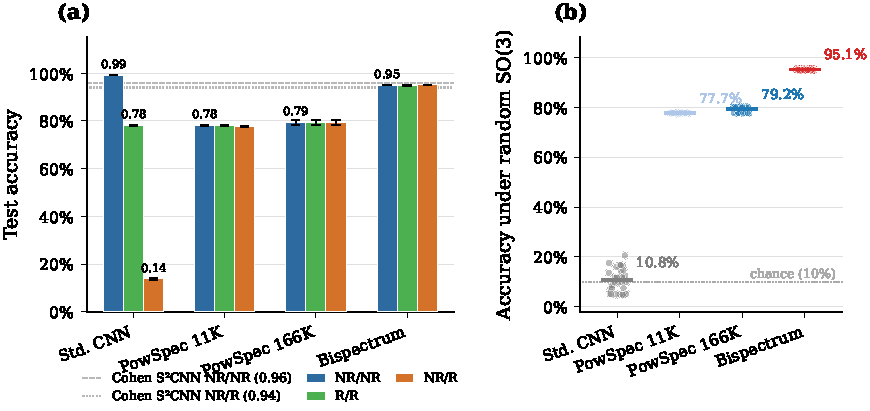
\includegraphics[width=0.9\linewidth]{experiments/spherical_mnist/smnist_analysis.pdf}
  \caption{Completeness, not capacity, drives the accuracy gap.
    \textbf{(a)}~The bispectrum nearly matches Cohen's spherical CNN
    across all protocols; the power spectrum plateaus ${\sim}17$pp lower.
    \textbf{(b)}~Under random $\SO(3)$ rotations, scaling the power
    spectrum MLP from 11K to 166K yields only ${+}1.4$pp.}
  \label{fig:smnist-analysis}
\end{figure}


\section{Discussion and Conclusion}
\label{sec:discussion}

We have presented \texttt{bispectrum}, a PyTorch library that makes
selective $G$-bispectral invariants practical, covering seven
group actions through a uniform \texttt{nn.Module} interface.
 We contribute a $\Theta(L^2)$ selective $\SO(3)$ invariant on
$S^2$ (Section~\ref{sec:so3-selective}). The selective forward pass
adds negligible overhead ($<$1\,ms for finite-group modules) and
delivers numerically exact rotation invariance with a consistent
data-efficiency advantage over incomplete alternatives in the
low-data/moderate-capacity regime.

\paragraph{When not to use the bispectrum.}
At high model capacity (Sec.~\ref{sec:experiments}), incomplete
alternatives like max pooling can match or surpass bispectral
pooling; each module is invariant to a \emph{specific} group
only. Data augmentation or flexible-symmetry equivariant networks
fit better when the relevant symmetry is multi-group or unknown.

\paragraph{Limitations and future work.}
Inversion from $\Phi_{\mathrm{sel}}$ is not shipped as a library
API, and a formal completeness proof, a characterization of the
degenerate set, and numerical-conditioning analysis at large
band-limits remain open. We do not compare against tensor-product
architectures (e3nn, MACE~\citep{batatia2022mace}) or wavelet scattering.

\begin{ack}
Omitted for review.
\end{ack}

\bibliographystyle{plainnat}
\bibliography{references}

\appendix

\section{Selective $\SO(3)$ Bispectrum -- Structural Background}
\label{app:so3-proof}

This appendix gives the structural background for the construction
of Section~\ref{sec:so3-selective}: the $S^2$ band-limited setup and
notation (Section~\ref{sec:app-setup}); the orbit-space dimension
lower bound $(L{+}1)^2-3$ that motivates the $\Theta(L^2)$ target
(Section~\ref{sec:app-lower-bound}); the explicit selective index set
together with the implementation-grade BFS variant
(Algorithm~\ref{alg:so3-augmented}) and per-degree counting result
(Section~\ref{sec:app-selective-index}); and the parity structure of
the scalar bispectrum that dictates the exclusion of certain
odd-parity triples in $\mathcal{T}_\ell$
(Section~\ref{sec:app-parity}). A short comparison with prior bispectral
constructions (Section~\ref{sec:app-comparison}) and a pixel-space
complexity table (Section~\ref{sec:app-pixel-complexity}) close the
appendix. We do not claim a closed-form completeness proof in this
revision; the empirical reconstruction of
Figure~\ref{fig:so3-reconstruction} is the proof-of-concept evidence
on which the construction is supported.

Per-degree entry allocation: the full seed
$\mathcal{S}_{\mathrm{seed}}$ handles $\ell\le L_{\mathrm{seed}}=4$
in constant size; for $\ell\ge 5$, Algorithm~\ref{alg:so3-augmented}
allocates $2\ell{+}1$ bispectral rows plus $O(\ell)$
self-coupling and CG-power entries, giving
$|\Phi_{\mathrm{sel}}|=\Theta(L^2)$ total (matching the orbit-space
lower bound $(L{+}1)^2-3$ of
Proposition~\ref{prop:app-lower-bound}; exact per-$L$ counts in
Table~\ref{tab:app-counts}).

\subsection{Setup and notation}
\label{sec:app-setup}

\begin{definition}[Band-limited signal on $S^2$]
A signal $f : S^2 \to \R$ is \emph{band-limited} at degree $L$ if its
spherical harmonic expansion
\begin{equation}\label{eq:app-sh-expansion}
  f(\theta, \varphi)
  = \sum_{\ell=0}^{L} \sum_{m=-\ell}^{\ell}
    a_\ell^m \, \SH_\ell^m(\theta, \varphi)
\end{equation}
has $a_\ell^m = 0$ for all $\ell > L$. We write
$\mathbf{F}_\ell = (a_\ell^{-\ell}, \dotsc, a_\ell^{\ell})
  \in \C^{2\ell+1}$
for the coefficient vector at degree~$\ell$.
\end{definition}

\noindent
For real $f$, the conjugation symmetry
$a_\ell^{-m} = (-1)^m \conj{a_\ell^m}$ holds, so
$\mathbf{F}_\ell$ has $2\ell+1$ real degrees of freedom.
The total signal dimension is
$\dim = \sum_{\ell=0}^{L}(2\ell+1) = (L+1)^2$.

\begin{definition}[Rotation action]
Under $g \in \SO(3)$, the spherical harmonic coefficients transform as
$\mathbf{F}_\ell \mapsto D^\ell(g)\,\mathbf{F}_\ell$,
where $D^\ell$ is the $(2\ell+1)$-dimensional Wigner~$D$-matrix.
\end{definition}

\noindent
In the irrep notation of~\citet{mataigne2024selective},
$\{\rho_\ell\}_{\ell\ge 0}$ are the (unitary) irreducible
representations of $\SO(3)$ with $V_{\rho_\ell}$ the
$(2\ell{+}1)$-dimensional space of degree-$\ell$ spherical harmonics
and $\rho_\ell(g)=D^\ell(g)$; the Fourier coefficient of $f$ at
$\rho_\ell$ is $\mathcal{F}(f)_{\rho_\ell}=\mathbf{F}_\ell$. We use
$\mathbf{F}_\ell$ as the working symbol throughout.

\begin{definition}[Bispectrum on $S^2$]\label{def:app-bispectrum}
For each triple $(\ell_1, \ell_2, \ell)$ satisfying the triangle
inequality $\abs{\ell_1 - \ell_2} \le \ell \le \ell_1 + \ell_2$,
the \emph{bispectral coefficient} is
\begin{equation}\label{eq:app-bispectrum}
  \beta_{\ell_1,\ell_2,\ell}
  = \sum_{\substack{m_1,\,m_2,\,m \\ m_1+m_2=m}}
    \CG{\ell_1}{m_1}{\ell_2}{m_2}{\ell}{m}\;
    a_{\ell_1}^{m_1}\,a_{\ell_2}^{m_2}\,\conj{a_\ell^m},
\end{equation}
where $\CG{\ell_1}{m_1}{\ell_2}{m_2}{\ell}{m}$ denotes the
Clebsch--Gordan coefficient
$\langle \ell_1, m_1;\, \ell_2, m_2 \mid \ell, m \rangle$.
Each $\beta_{\ell_1,\ell_2,\ell}$ is a scalar; for real~$f$ it is
real when $\ell_1{+}\ell_2{+}\ell$ is even and purely imaginary when
$\ell_1{+}\ell_2{+}\ell$ is odd (Lemma~\ref{lem:app-parity}).
\end{definition}

Definition~\ref{def:app-bispectrum} is the specialization of the
general $G$-bispectrum (eq.~\eqref{eq:bispectrum-def}) to the case
$G = \SO(3)$ acting on~$S^2$, where the irreps are Wigner-$D$
matrices and the Fourier coefficients are spherical harmonic
coefficients~$a_\ell^m$.

\begin{definition}[CG power spectrum, optional diagnostic]\label{def:app-cg-power}
For a triple $(\ell_1, \ell_2, \ell)$ satisfying the triangle
inequality, write
$(\mathbf{F}_{\ell_1} \otimes \mathbf{F}_{\ell_2})\big|_\ell$
for the projection of the Kronecker product
$\mathbf{F}_{\ell_1} \otimes \mathbf{F}_{\ell_2}$ onto the
$D^\ell$-isotypic component, realised by contracting with the CG
coefficients $\CG{\ell_1}{m_1}{\ell_2}{m_2}{\ell}{m}$. The
\emph{CG power spectrum entry} is the squared norm of this projection,
\begin{equation}\label{eq:app-cg-power}
  P_{\ell_1,\ell_2,\ell}
  := \lVert (\mathbf{F}_{\ell_1} \otimes \mathbf{F}_{\ell_2})|_\ell
     \rVert^2
  = \sum_{m=-\ell}^{\ell}
    \Bigl\lvert \sum_{\substack{m_1,m_2 \\ m_1+m_2=m}}
      \CG{\ell_1}{m_1}{\ell_2}{m_2}{\ell}{m}\;
      a_{\ell_1}^{m_1}\, a_{\ell_2}^{m_2} \Bigr\rvert^2.
\end{equation}
This is a degree-$4$, real-valued, $\SO(3)$-invariant polynomial in
the signal coefficients. The library appends a $O(L^2)$ family of CG
power scalars to the selective bispectrum unconditionally for
numerical robustness on the real-signal slice
(Remark~\ref{rem:app-Tell-rank-deficit}); they leave the asymptotic
output size unchanged.
\end{definition}

\begin{proposition}[Size of the full bispectrum]\label{prop:app-full-size}
The number of admissible triples $(\ell_1, \ell_2, \ell)$ with
$0 \le \ell_1, \ell_2, \ell \le L$ satisfying the triangle inequality
$|\ell_1 - \ell_2| \le \ell \le \ell_1 + \ell_2$ is $\Theta(L^3)$.
\end{proposition}
\begin{proof}
For fixed $\ell_1$ and $\ell_2$, the triangle inequality admits
$\min(\ell_1 + \ell_2, L) - |\ell_1 - \ell_2| + 1$ valid values of
$\ell$. Summing over $(\ell_1,\ell_2)\in[0,L]^2$ gives
$N_{\mathrm{full}} = \Theta(L^3)$.
\end{proof}

\begin{remark}[Invariance]
Each $\beta_{\ell_1,\ell_2,\ell}$ is $\SO(3)$-invariant: the Wigner
matrices satisfy $D^{\ell_1} \otimes D^{\ell_2}
= \bigoplus_\ell D^\ell$ under the CG decomposition, so the triple
product contracted with CG coefficients is unchanged by
$\mathbf{F}_\ell \mapsto D^\ell(g)\mathbf{F}_\ell$.
\end{remark}

\subsection{Why $\mathcal{O}(L)$ is impossible}
\label{sec:app-lower-bound}

\begin{proposition}[Dimensional lower bound]\label{prop:app-lower-bound}
Any \emph{smooth or polynomial} complete $\SO(3)$-invariant for
band-limited signals on $S^2$ at band-limit $L$ must have codomain
of dimension at least $(L+1)^2 - 3$.
\end{proposition}
\begin{proof}
Let $\Phi : \R^{(L+1)^2} \to \R^k$ be a smooth (or polynomial)
$\SO(3)$-invariant map that separates orbits on a Zariski-open
dense subset $U\subset\R^{(L+1)^2}$. Smoothness implies $\Phi$ has a
well-defined generic rank $r := \max_{x\in U} \mathrm{rank}\,
d\Phi_x$; on the open dense subset where this rank is attained,
$\Phi$ is locally a submersion onto an $r$-dimensional submanifold,
and orbit-separation forces $r \ge \dim(\R^{(L+1)^2}/\SO(3))
= (L+1)^2 - \dim\SO(3) = (L+1)^2 - 3$
(generic-rank theorem for $\SO(3)$ acting on $V_L$;
cf.~Tarski--Seidenberg in the polynomial case). Hence
$k \ge r \ge (L+1)^2 - 3 = \Omega(L^2)$.
\end{proof}

\begin{remark}
The chain $\beta_{1,\ell,\ell+1}$ for $\ell = 0, \dotsc, L-1$ provides
only $\sim 3L$ scalar constraints (since each chain entry couples
$\mathbf{F}_1 \in \C^3$ with one known $\mathbf{F}_\ell$). This cannot
recover $(L+1)^2 \approx L^2$ unknowns.
\end{remark}

\begin{remark}[Smoothness assumption]
The smoothness/polynomial qualifier is essential: pathological
non-measurable invariants (e.g.\ a fixed orbit-section indexed by
the axiom of choice) can in principle have codomain dimension $1$
but are not implementable. All practical bispectral or spectral
invariants are polynomial, so the proposition applies.
\end{remark}

\subsection{The selective index set}
\label{sec:app-selective-index}

For each target degree $\ell$, the library's selective invariant
allocates $2\ell{+}1$ linear bispectral entries, plus quadratic/cubic
self-couplings and CG-power scalars for numerical robustness on the
real-signal slice. Combined with a constant-size full-bispectrum seed
at degrees $\le L_{\mathrm{seed}}=\min(L,4)$, this gives an
$O(L^2)$-sized invariant matching the orbit-space lower bound of
Proposition~\ref{prop:app-lower-bound}.

\begin{definition}[Augmented selective $\SO(3)$-on-$S^2$ invariant]\label{def:app-selective}
Set $L_{\mathrm{seed}} := \min(L,4)$. Let
$\mathcal{S}_{\mathrm{seed}}$ denote the bispectral triples at
degrees $\ell\le L_{\mathrm{seed}}$ returned by
Algorithm~\ref{alg:so3-augmented}'s seed phase: the pre-prune set
collects all admissible triples
$\{(\ell_1,\ell_2,\ell):
0\le\ell_1\le\ell_2\le L_{\mathrm{seed}},\,
|\ell_1{-}\ell_2|\le\ell\le\min(\ell_1{+}\ell_2,L_{\mathrm{seed}})\}$
($42$ triples at $L_{\mathrm{seed}}=4$); Algorithm~\ref{alg:so3-augmented}
then parity-prunes entries that vanish identically on real signals
(Lemma~\ref{lem:app-parity}), deduplicates, and caps each degree
to its per-degree budget. The surviving bispectral count at $L=4$
is $24$ (see Table~\ref{tab:app-counts}, column ``Bispectral''),
and $|\mathcal{S}_{\mathrm{seed}}|$ is constant in $L$ for $L\ge 4$.
For each intermediate target $4\le\ell\le 7$ Algorithm~\ref{alg:so3-augmented}
uses the small explicit linear block $\mathcal{T}_\ell^{\mathrm{small}}$
(Table~\ref{tab:Tsmall}); for each high-degree target $\ell\ge 8$
the \emph{bootstrap block} $\mathcal{T}_\ell$ is
\begin{equation}\label{eq:app-Tell}
\begin{aligned}
  \mathcal{T}_\ell
  := &\ \{(a,\ell,\ell-a) : 1\le a \le \ell{-}1\} \\
   &\cup \bigl\{(a,\ell,\ell-a+1) : 2\le a \le \ell{-}1,
        \; a \ne (\ell+1)/2 \bigr\} \\
   &\cup \{(a,\ell-a,\ell) : 1\le a \le 4\} \;\cup\; \mathcal{Z}_\ell,
\end{aligned}
\end{equation}
where $\mathcal{Z}_\ell = \emptyset$ for even $\ell$ and
$\mathcal{Z}_\ell = \{(2,\ell{-}1,\ell)\}$ for odd $\ell\ge 9$. The
exclusion $a\ne (\ell+1)/2$ for odd $\ell$ removes the self-conjugate
triple $(r,2r-1,r)$ at $\ell = 2r-1$, which has a repeated index and
vanishes identically on real signals
(Proposition~\ref{prop:app-odd-vanishing}); the compensating row
$(2,\ell{-}1,\ell)\in\mathcal{Z}_\ell$ has all-distinct indices and
does not overlap the chain family (which only covers pairs
$(a,\ell{-}a)$ with $a\le 4$). Size bookkeeping:
$(\ell{-}1)+(\ell{-}2)+4 = 2\ell{+}1$ for even $\ell$, and
$(\ell{-}1)+(\ell{-}3)+4+1 = 2\ell{+}1$ for odd $\ell\ge 9$; the first
two families differ in the last index ($\ell{-}a$ vs.\ $\ell{-}a+1$),
and $\mathcal{Z}_\ell$ at $a=2$ has second coordinate $\ell{-}1$
rather than $\ell{-}2$, so all three subfamilies are disjoint.

The \emph{augmented selective $\SO(3)$-on-$S^2$ invariant}
$\Phi_{\mathrm{sel}}$ is the output of
Algorithm~\ref{alg:so3-augmented}: bispectral triples
$\mathcal{S}_\beta = \mathcal{S}_{\mathrm{seed}}\cup
\bigcup_{\ell=5}^{L}\mathcal{T}_\ell$ (with
$\mathcal{T}_\ell = \mathcal{T}_\ell^{\mathrm{small}}$ for
$5\le\ell\le 7$), mandatory even self-couplings
$\beta_{\ell,\ell,\ell'}$ ($\ell'$ even, $2\le\ell'\le\ell$), and
CG-power scalars $P_{\ell_1,\ell_2,\ell} = \lVert(\mathbf{F}_{\ell_1}
\otimes \mathbf{F}_{\ell_2})|_\ell\rVert^2$
(Definition~\ref{def:app-cg-power}) chosen greedily for per-degree
Jacobian rank. Mathematically, $\Phi_{\mathrm{sel}}:V_L\to\R^N$ has
$N$ live real scalar components: by
Lemma~\ref{lem:app-parity}, each bispectral entry contributes one
real component on the real-signal slice (real for even parity,
purely imaginary for odd), and CG-power entries are real-valued
degree-$4$ invariants. The PyTorch implementation stores each
scalar in a complex tensor, so downstream layers receive $2N$ real
channels after splitting real and imaginary parts; for bispectral
entries exactly one of the two channels is structurally zero by
parity, and for CG-power entries the imaginary channel is
structurally zero.
\end{definition}

\begin{table}[h]
  \caption{Explicit low-degree bootstrap blocks
    $\mathcal{T}_\ell^{\mathrm{small}}$ for $4\le\ell\le 7$, copied
    from \texttt{bispectrum.so3\_on\_s2.\_small\_linear\_bootstrap\_block}.
    Each triple $(\ell_1,\ell_2,\ell_3)$ denotes
    $\beta_{\ell_1,\ell_2,\ell_3}$; all are admissible and have
    $\ell$ in at least one slot. Entry counts
    $|\mathcal{T}_4^{\mathrm{small}}|=10$,
    $|\mathcal{T}_5^{\mathrm{small}}|=11$,
    $|\mathcal{T}_6^{\mathrm{small}}|=13$,
    $|\mathcal{T}_7^{\mathrm{small}}|=15$ match the per-degree budgets.
    $\mathcal{T}_4^{\mathrm{small}}$ is implementation-only:
    Algorithm~\ref{alg:so3-augmented} uses it as a ranked candidate
    list at $\ell=4$, deduplicated against the seed
    $\mathcal{S}_{\mathrm{seed}}$ and capped to a budget of $10$ entries;
    $\mathcal{T}_5^{\mathrm{small}},\mathcal{T}_6^{\mathrm{small}},\mathcal{T}_7^{\mathrm{small}}$
    are the formal bootstrap blocks at $\ell\in\{5,6,7\}$.}
  \label{tab:Tsmall}
  \centering
  \small
  \setlength{\tabcolsep}{4pt}
  \footnotesize
  \begin{tabular}{@{}cp{0.92\linewidth}@{}}
    \toprule
    $\ell$ & $\mathcal{T}_\ell^{\mathrm{small}}$ (each entry a triple $(\ell_1,\ell_2,\ell_3)$) \\
    \midrule
    $4$ & $(1,3,4),$ $(2,2,4),$ $(2,3,4),$ $(3,3,4),$ $(1,4,3),$ $(2,4,2),$ $(3,4,1),$ $(2,4,3),$ $(3,4,2),$ $(3,4,3)$ \\
    $5$ & $(1,4,5),$ $(2,3,5),$ $(2,4,5),$ $(3,4,5),$ $(1,5,4),$ $(2,5,3),$ $(3,5,2),$ $(4,5,1),$ $(2,5,4),$ $(3,5,4),$ $(4,5,4)$ \\
    $6$ & $(1,5,6),$ $(2,4,6),$ $(3,3,6),$ $(3,4,6),$ $(1,6,5),$ $(2,6,4),$ $(3,6,3),$ $(4,6,2),$ $(5,6,1),$ $(2,6,5),$ $(3,6,5),$ $(4,6,5),$ $(5,6,5)$ \\
    $7$ & $(1,6,7),$ $(2,5,7),$ $(3,4,7),$ $(4,5,7),$ $(1,7,6),$ $(2,7,5),$ $(3,7,4),$ $(4,7,3),$ $(5,7,2),$ $(6,7,1),$ $(2,7,6),$ $(3,7,6),$ $(4,7,6),$ $(5,7,6),$ $(6,7,6)$ \\
    \bottomrule
  \end{tabular}
\end{table}

\begin{table}[h]
  \caption{Coefficient counts of $\Phi_{\mathrm{sel}}$ at
    representative band-limits. ``Bispectral'' counts the triples in
    $\mathcal{S}_\beta$ (including mandatory even self-couplings);
    ``CG-power'' counts entries in $\mathcal{S}_P$; ``Total $N$'' is
    $|\Phi_{\mathrm{sel}}|$ (live real components) and matches the
    library's \texttt{output\_size}. ``Stored channels'' counts the
    complex-tensor storage ($2N$) seen by the SMNIST classifier;
    one channel per bispectral entry is structurally zero by
    parity, and the imaginary channel of each CG-power entry is
    structurally zero.}
  \label{tab:app-counts}
  \centering
  \small
  \setlength{\tabcolsep}{6pt}
  \begin{tabular}{ccccc}
    \toprule
    $L$ & Bispectral & CG-power & Total $N=|\Phi_{\mathrm{sel}}|$
        & Stored channels ($2N$) \\
    \midrule
    $4$  & $24$  & $10$  & $34$  & $68$  \\
    $5$  & $37$  & $17$  & $54$  & $108$ \\
    $15$ & $307$ & $77$  & $384$ & $768$ \\
    $16$ & $348$ & $82$  & $430$ & $860$ \\
    \bottomrule
  \end{tabular}
\end{table}
\clearpage
\begin{algorithm}[H]
\caption{Augmented selective index set for the $\SO(3)$ bispectrum
  on $S^2$ at band-limit~$L$. Returns bispectral triples
  $\mathcal{S}_\beta$ and CG power triples $\mathcal{S}_P$.
  This extends the BFS-based selective index construction of
  \citet{mataigne2024selective} from finite groups to $\SO(3)$ on $S^2$,
  adding the CG power augmentation step that is specific to real
  signals.}
\label{alg:so3-augmented}
\small
\begin{algorithmic}[1]
\STATE \textbf{Input:} Band-limit $L$
\STATE \textbf{Output:} Bispectral set $\mathcal{S}_\beta$, CG power
  set $\mathcal{S}_P$
\STATE $\mathcal{S}_\beta \leftarrow \{(0,0,0)\}$;
  $\mathcal{S}_P \leftarrow \emptyset$
\STATE \textbf{Seed block:} add to $\mathcal{S}_\beta$ all triples
  $(\ell_1, \ell_2, \ell)$ with $0 \le \ell_1 \le \ell_2 \le L_0 = 4$
  and $|\ell_1 - \ell_2| \le \ell \le \min(\ell_1 + \ell_2, L_0)$
  \COMMENT{constant-size full-bispectrum seed}
\FOR{$\ell = 1, \dotsc, L$}
  \STATE $\text{budget} \leftarrow 2\ell + 1$
  \IF{$\ell = 4$}
    \STATE $\text{budget} \leftarrow 10$
      \COMMENT{keep all chain+cross at $\ell=4$}
  \ENDIF
  \STATE $\text{candidates} \leftarrow [\,]$
  \IF{$4 \le \ell \le 7$}
    \STATE append the explicit low-degree linear block
      $\mathcal{T}^{\mathrm{small}}_\ell$ to candidates
  \ELSIF{$\ell \ge 8$}
    \FOR{$a = 1, \dotsc, \ell{-}1$}
      \STATE append $(a,\, \ell,\, \ell{-}a)$ to candidates
    \ENDFOR
    \FOR{$a = 2, \dotsc, \ell{-}1$}
      \IF{\NOT ($\ell$ is odd \AND $a = (\ell{+}1)/2$)}
        \STATE append $(a,\, \ell,\, \ell{-}a{+}1)$ to candidates
          \COMMENT{skip $(r,2r{-}1,r)\equiv0$ on real signals,
            Prop.~\ref{prop:app-odd-vanishing}}
      \ENDIF
    \ENDFOR
    \FOR{$a = 1, \dotsc, 4$}
      \STATE append $(a,\, \ell{-}a,\, \ell)$ to candidates
    \ENDFOR
    \IF{$\ell$ is odd}
      \STATE append $(2,\, \ell{-}1,\, \ell)$ to candidates
        \COMMENT{compensate excluded $(r,2r{-}1,r)$ row}
    \ENDIF
  \ELSE
    \STATE append low-degree chain candidates
    \IF{$\ell \ne 2$}
      \STATE append cross candidates
        \COMMENT{$\beta_{1,2,1}$ excluded}
    \ENDIF
  \ENDIF
  \STATE append $(0,\, \ell,\, \ell)$ to candidates
    \COMMENT{power entry}
  \IF{$\ell \notin \{1,\, 2\}$}
    \FOR{$\ell' = \ell{-}1, \dotsc, 0$}
      \STATE append $(\ell,\, \ell,\, \ell')$ to candidates
    \ENDFOR
  \ENDIF
  \IF{$\ell = 2$}
    \STATE append $(\ell,\, \ell,\, \ell)$ to candidates
      \COMMENT{$\beta_{2,2,2}$}
  \ENDIF
  \STATE Remove entries that vanish for real signals; deduplicate
    against $\mathcal{S}_\beta$ already added by the seed block
  \STATE $\mathcal{S}_\beta \leftarrow \mathcal{S}_\beta
    \;\cup\;$ first $\min(\text{budget},\,
    |\text{candidates}|)$ live entries
  \STATE \COMMENT{\textbf{Mandatory even self-couplings}}
  \FOR{$\ell' = 2, 4, \dotsc, \lfloor\ell/2\rfloor \cdot 2$
    with $\ell' \le \ell$ and $\ell \ge 3$}
    \STATE $\mathcal{S}_\beta \leftarrow \mathcal{S}_\beta
      \cup \{(\ell,\, \ell,\, \ell')\}$
  \ENDFOR
  \STATE \COMMENT{\textbf{CG power augmentation}}
  \STATE Greedily add $P_{\ell_1,\ell_2,\ell'}$ (with
    $\max(\ell_1,\ell_2) = \ell$, $|\ell_1{-}\ell_2| \le \ell'
    \le \ell_1{+}\ell_2$) to $\mathcal{S}_P$ until the
    Jacobian rank of the per-degree restriction
    $\Phi_{\mathrm{sel}}|_\ell$ matches the number of unknowns
\ENDFOR
\RETURN $(\mathcal{S}_\beta,\, \mathcal{S}_P)$
\end{algorithmic}
\end{algorithm}

\begin{proposition}[Output size]\label{prop:app-output-size}
For every $L\ge 4$, Algorithm~\ref{alg:so3-augmented} produces a
$\Theta(L^2)$-sized invariant: the per-degree bootstrap block
contributes at most $2\ell{+}1$ bispectral triples
(Eq.~\eqref{eq:app-Tell} for $\ell\ge 8$ plus
Table~\ref{tab:Tsmall} for $5\le\ell\le 7$), and the self-coupling
and CG-power augmentations add $O(\ell)$ per degree, giving a total
of $\Theta(L^2)$ real scalars. Per-$L$ counts are listed in
Table~\ref{tab:app-counts}; both panels match the orbit-space
lower bound $(L{+}1)^2-3$ of Proposition~\ref{prop:app-lower-bound}
up to a constant factor.
\end{proposition}



\subsection{Parity structure of the bispectrum}
\label{sec:app-parity}

The selective construction of Section~\ref{sec:so3-selective}
exploits two structural facts about the scalar bispectrum
$\beta_{\ell_1,\ell_2,\ell}$: a parity rule that fixes whether each
entry is real or purely imaginary on real signals (Lemma~\ref{lem:app-parity})
and the resulting identical vanishing of certain odd-parity entries
with a repeated index (Proposition~\ref{prop:app-odd-vanishing}). The
latter dictates the explicit exclusion in $\mathcal{T}_\ell$ at odd
target degrees, and the former is the source of the rank deficit
that motivates the CG-power augmentation of
Algorithm~\ref{alg:so3-augmented} (Remark~\ref{rem:app-Tell-rank-deficit}).

\begin{lemma}[Parity of the bispectrum]\label{lem:app-parity}
For any signal (real or complex):
\begin{equation}\label{eq:app-parity}
  \beta_{\ell_1,\ell_2,\ell}(T_R \cdot f)
  = (-1)^{\ell_1+\ell_2+\ell}\,\beta_{\ell_1,\ell_2,\ell}(f).
\end{equation}
For \emph{real} signals, there is an independent constraint:
\begin{equation}\label{eq:app-reality-constraint}
  \conj{\beta_{\ell_1,\ell_2,\ell}(f)}
  = (-1)^{\ell_1+\ell_2+\ell}\,\beta_{\ell_1,\ell_2,\ell}(f).
\end{equation}
Together:
\begin{enumerate}[nosep,label=(\alph*)]
\item If $\ell_1+\ell_2+\ell$ is even:
  $\beta$ is real-valued (by~\eqref{eq:app-reality-constraint})
  and $T_R$-invariant (by~\eqref{eq:app-parity}).
\item If $\ell_1+\ell_2+\ell$ is odd:
  $\beta$ is purely imaginary (by~\eqref{eq:app-reality-constraint})
  and $\beta(T_R \cdot f) = -\beta(f)$, so $\im\beta$ flips sign under $T_R$.
\end{enumerate}
\end{lemma}
\begin{proof}
Under $T_R$, each $a_\ell^m \mapsto (-1)^m a_\ell^{-m}$.
Substituting into $\beta = \sum_m (\sum_{m_1+m_2=m} C\, a^{m_1} a^{m_2})
\conj{a^m}$, the three sign factors $(-1)^{m_1+m_2+m} = (-1)^{2m} = 1$
cancel. Re-indexing $m \mapsto -m$ and applying the CG symmetry
$\CG{\ell_1}{-m_1}{\ell_2}{-m_2}{\ell}{-m}
  = (-1)^{\ell_1+\ell_2-\ell}\,\CG{\ell_1}{m_1}{\ell_2}{m_2}{\ell}{m}$
yields~\eqref{eq:app-parity} (with $(-1)^{\ell_1+\ell_2-\ell} = (-1)^{\ell_1+\ell_2+\ell}$).

For real signals, $\conj{a_\ell^m} = (-1)^m a_\ell^{-m}$.
Taking the complex conjugate of $\beta$ and re-indexing similarly
yields~\eqref{eq:app-reality-constraint}.
\end{proof}

\begin{lemma}[CG power is $T_R$-invariant]\label{lem:app-P-invariant}
For all triples $(\ell_1,\ell_2,\ell)$:
$P_{\ell_1,\ell_2,\ell}(T_R \cdot f) = P_{\ell_1,\ell_2,\ell}(f)$.
\end{lemma}
\begin{proof}
Under $T_R$, the CG-projected component transforms as
$(\mathbf{F}_{\ell_1} \otimes \mathbf{F}_{\ell_2})|_\ell^M
  \mapsto (-1)^{\ell_1+\ell_2+\ell+M}\,
  (\mathbf{F}_{\ell_1} \otimes \mathbf{F}_{\ell_2})|_\ell^{-M}$.
Taking the squared norm and re-indexing the sum over $M$
leaves $P$ unchanged.
\end{proof}

\begin{proposition}[Vanishing of odd-parity entries with a repeated index]
\label{prop:app-odd-vanishing}
Let $\beta_{\ell_1,\ell_2,\ell}$ be the scalar bispectrum entry of a
real signal $f$ (so $\ell_1+\ell_2+\ell$ odd). If the index multiset
$\{\ell_1,\ell_2,\ell\}$ contains a repeated value, then
$\beta_{\ell_1,\ell_2,\ell}(f)\equiv 0$ as a polynomial in the SH
coefficients of $f$.
\end{proposition}

\begin{proof}
Define the symmetric scalar 3j contraction
\[
  T_{\ell_1,\ell_2,\ell_3}(f) :=
  \sum_{m_1,m_2,m_3}
  \begin{pmatrix} \ell_1 & \ell_2 & \ell_3 \\
                  m_1 & m_2 & m_3 \end{pmatrix}\,
  a_{\ell_1}^{m_1}\, a_{\ell_2}^{m_2}\, a_{\ell_3}^{m_3} .
\]
Converting the Wigner~3j into a Clebsch-Gordan coefficient via
$\bigl(\begin{smallmatrix} j_1 & j_2 & j_3 \\
       m_1 & m_2 & m_3\end{smallmatrix}\bigr)
= \frac{(-1)^{j_1-j_2-m_3}}{\sqrt{2j_3+1}}\,
  \CG{j_1}{m_1}{j_2}{m_2}{j_3}{-m_3}$ and applying the reality identity
$a_{\ell_3}^{m_3} = (-1)^{m_3}\,\conj{a_{\ell_3}^{-m_3}}$ shows
\[
  \beta_{\ell_1,\ell_2,\ell}(f)
  = (-1)^{\ell_1+\ell_2}\sqrt{2\ell+1}\,
    T_{\ell_1,\ell_2,\ell}(f),
\]
so $\beta$ and $T$ have the same vanishing locus. The 3j symbol is
invariant under even column permutations and picks up
$(-1)^{\ell_1+\ell_2+\ell_3}$ under odd ones. If two columns $i,j$
satisfy $\ell_i=\ell_j$, the inserted vectors $a_{\ell_i},a_{\ell_j}$
are literally the same coefficient vector of $f$, so swapping those
two columns leaves the contracted sum $T$ unchanged while multiplying
the 3j prefactor by $(-1)^{\ell_1+\ell_2+\ell_3}$. For odd parity this
forces $T=-T$, hence $T\equiv 0$ and $\beta\equiv 0$.
\end{proof}

\begin{remark}[Consequences for $\mathcal{T}_\ell$]
\label{rem:app-Tell-zero-rows}
Proposition~\ref{prop:app-odd-vanishing} applies in particular to the
family $(r,2r-1,r)$: it has parity $4r-1$ (odd) and a repeated index,
so $\beta_{r,2r-1,r}\equiv 0$ on real signals. Numerical evaluation at
the seed-42 real witness confirms this: for $r=2,\dots,7$ the entry is
zero to double-precision rounding ($|\beta|\lesssim 10^{-14}$). Any
formal definition of $\mathcal{T}_\ell$ must therefore exclude these
triples (see~\eqref{eq:app-Tell}); we substitute a chain row with
all-distinct indices in their place.
\end{remark}

\begin{corollary}[First nonzero odd-parity entry]\label{cor:app-first-odd}
The first bispectral entry with odd parity and generically nonzero imaginary
part occurs at degree $\ell = 4$:
$\beta_{2,3,4}$, with
$\ell_1+\ell_2+\ell = 9$ (odd) and
$\ell_1, \ell_2, \ell$ all distinct.
At the deterministic witness (seed~42), $\im(\beta_{2,3,4}) \approx 3.26 \ne 0$,
and $\im(\beta_{2,3,4})(T_R \cdot f) \approx -3.26$.
Similarly, $\beta_{2,4,3}$ and $\beta_{3,4,2}$ are nonzero odd-parity entries
at degree~$4$.
\end{corollary}

\begin{remark}[No parity-breaking at $\ell \le 3$]\label{rem:app-no-parity-breaking-le3}
For degrees $\le 3$, every odd-parity triple $(\ell_1,\ell_2,\ell)$
has at least two indices equal (since $\max(\ell_1,\ell_2,\ell) \le 3$
and $\ell_1+\ell_2+\ell$ odd forces at least one pair to be equal in this range).
By Proposition~\ref{prop:app-odd-vanishing}, all odd-parity entries vanish.
Therefore, the $T_R$ ambiguity cannot be resolved using only degrees $\le 3$.
\end{remark}

\begin{remark}[Why the augmented block is needed]
\label{rem:app-Tell-rank-deficit}
The bootstrap block $\mathcal{T}_\ell$ alone is rank-deficient on the
real-signal slice: at the seed-42 real witness, the
$(2\ell{+}1)\times(2\ell{+}1)$ submatrix $A_\ell$ assembled from the
$\mathcal{T}_\ell$ rows has SVD rank
$\approx \ell{+}2$ rather than $2\ell{+}1$ for $\ell\in\{8,\dots,15\}$
(verified numerically; the deficit is generic over real witnesses).
The mandatory even self-couplings and CG-power scalars are quadratic
or cubic in $\mathbf{F}_\ell$ and supply the additional independent
real equations needed to fill out the per-degree real Jacobian; the
augmented per-degree block (linear $\mathcal{T}_\ell$ plus quadratic
self-couplings plus CG-power scalars) is what
Algorithm~\ref{alg:so3-augmented} assembles, and is what the
implementation actually solves at degrees $\ell\ge 5$.
\end{remark}

\subsection{Comparison with existing results}
\label{sec:app-comparison}

\begin{table}[h]
  \caption{Comparison of bispectral invariants for signals on $S^2$ or
    finite groups.}
  \label{tab:app-comparison}
  \centering
  \small
  \setlength{\tabcolsep}{4pt}
  \begin{tabular}{@{}l l c c@{}}
    \toprule
    Result & Invariant & Size & Complete? \\
    \midrule
    Kakarala~\citep{kakarala2012bispectrum}
      & Full bispec. & $O(L^3)$ & Yes (constr.) \\
    Edidin \& Satriano~\citep{edidin2024orbit}
      & Full bispec.\ (band-lim.)
      & $O(L^3)$ & Yes (generic) \\
    Bendory et al.~\citep{bendory2025orbit}
      & Freq.\ marching
      & $O(L^2)$/shell & Yes (3~shells) \\
    Mataigne et al.~\citep{mataigne2024selective}
      & Sel.\ $G$-bispec.\ (finite)
      & $O(|G|)$ & Yes (exact) \\
    \textbf{This work}
      & \textbf{Sel.\ $\SO(3)$ on $S^2$}
      & $\boldsymbol{\Theta(L^2)}$
      & \textbf{Empirical (Section~\ref{sec:so3-recon})} \\
    \bottomrule
  \end{tabular}
\end{table}

\subsection{Complexity in pixel space}
\label{sec:app-pixel-complexity}

On $S^2$, a band-limited signal at degree~$L$ is sampled on an
equiangular grid of size $N_\theta \times N_\varphi \approx 2L \times 2L$,
so $P = 4L^2$ and $L = \Theta(\sqrt{P})$.

\paragraph{Output size.}
\begin{center}
\small
\begin{tabular}{lcc}
  \toprule
  Invariant & In $L$ & In $P$ \\
  \midrule
  Power spectrum & $O(L)$ & $O(\sqrt{P})$ \\
  \textbf{Selective bispectrum} & $\boldsymbol{O(L^2)}$
    & $\boldsymbol{O(P)}$ \\
  Full bispectrum & $O(L^3)$ & $O(P^{3/2})$ \\
  \bottomrule
\end{tabular}
\end{center}
The selective bispectrum is \emph{linear} in the number of pixels.

\paragraph{Computation cost.}
\begin{center}
\small
\begin{tabular}{lcccc}
  \toprule
  Variant & Entries & Cost/entry & Total & In $P$ \\
  \midrule
  Full & $O(L^3)$ & $O(L)$ & $O(L^4)$ & $O(P^2)$ \\
  Selective & $O(L^2)$ & $O(L)$ & $O(L^3)$ & $O(P^{3/2})$ \\
  \bottomrule
\end{tabular}
\end{center}

\paragraph{Concrete example.}
For a $128 \times 256$ grid ($P \approx 32\mathrm{K}$, $L = 64$): the
full bispectrum produces ${\sim}87\mathrm{K}$ scalars at
${\sim}17\mathrm{M}$~ops; the selective bispectrum produces
${\sim}4\mathrm{K}$ scalars at ${\sim}260\mathrm{K}$~ops---a
$65\times$ reduction.

\section{Extended Benchmark Results}
\label{app:bench}

This appendix supplements the summary in Table~\ref{tab:benchmarks}
(main text) with scaling plots produced by
\texttt{benchmarks/benchmark.py} on a single NVIDIA H100 80\,GB GPU
(PyTorch 2.10).

\subsection{Coefficient-count scaling}

\begin{figure}[h]
  \centering
  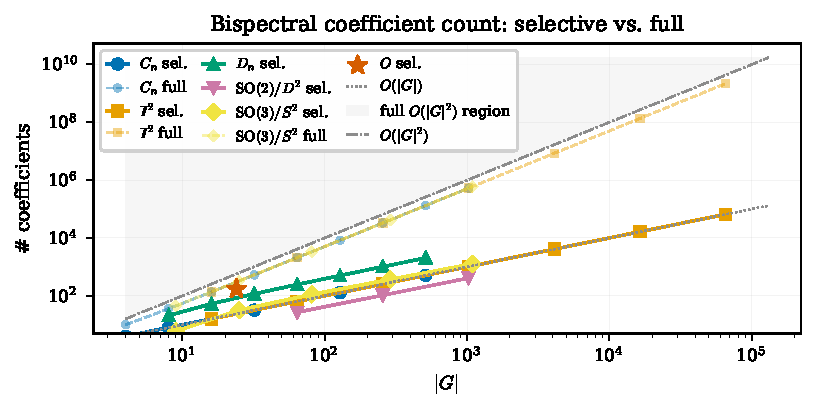
\includegraphics[width=\linewidth]{experiments/benchmarks/paper_fig1.pdf}
  \caption{Bispectral coefficient count vs.\ group order $|G|$. Solid
    lines: selective ($O(|G|)$); dashed: full ($O(|G|^2)$). At
    $|G|{=}1{,}024$, selectivity yields a $512\times$ reduction.
    Continuous groups ($\SO(2)$, $\SO(3)$) are plotted at their
    band-limited signal dimension; full-bispectrum curves for $D_n$
    and the disk are omitted (backends not yet implemented).}
  \label{fig:coeff-scaling}
\end{figure}

\subsection{Forward-pass timing}

\begin{figure}[h]
  \centering
  
\includegraphics[width=\linewidth]{experiments/benchmarks/paper_fig2.pdf}
  \caption{Forward-pass wall-clock time (batch\,=\,16, H100 GPU).
    \textbf{(a)}~$C_n$: the selective pass stays flat at
    ${\sim}$0.14\,ms regardless of $n$, while the full bispectrum
    grows super-linearly (17\,ms at $n{=}256$).
    \textbf{(b)}~$\mathbb{T}^2$: selective is constant at
    ${\sim}$0.08\,ms up to $|G|{=}65{,}536$.}
  \label{fig:forward-timing}
\end{figure}

The selective forward pass is dominated by kernel-launch overhead
rather than arithmetic, making it effectively free relative to backbone
computation. The full bispectrum exhibits the expected super-linear
growth and becomes impractical beyond $|G| \approx 256$ for $C_n$.

\subsection{GPU throughput and inversion}

\begin{figure}[h]
  \centering
  
\includegraphics[width=\linewidth]{experiments/benchmarks/paper_fig3.pdf}
  \caption{\textbf{(a)}~GPU throughput (samples/s) vs.\ batch size for
    the selective forward pass. $C_n$ and $\mathbb{T}^2$ exceed
    $10^7$~samples/s; the octahedral module reaches
    $5.7 \times 10^6$~samples/s. All modules scale linearly with batch
    size.
    \textbf{(b)}~Inversion wall-clock time. Abelian groups ($C_n$,
    $D_n$, $\SO(2)$/disk) scale roughly linearly. $\SO(3)$ on $S^2$
    inversion is not yet implemented.}
  \label{fig:gpu-scaling}
\end{figure}

All modules exhibit linear throughput scaling with batch size, confirming
that the implementation is memory-bandwidth-bound rather than
compute-bound at these scales.

\section{PCam: Extended Results}
\label{app:pcam-details}

\begin{table}[h]
  \caption{Accuracy of a $G$-bispectral pooling layer on PatchCamelyon (PCam)~\citep{veeling2018rotation}, a binary histopathology classification benchmark. $G$-bispectral pooling is competitive with classical pooling approaches.}
  \label{tab:pcam-results}
  \centering
  \small
  \begin{tabular}{lrcc}
    \toprule
    Model & Params & Test AUC & Test ACC \\
    \midrule
    Standard (data augmented)          & 102K & $.896 \pm .010$ & $.826 \pm .012$ \\
    Gated                         & 136K & $.941 \pm .009$ & $.870 \pm .004$ \\
    Selective Bispectrum (\texttt{CnonCn})  & 128K & $.941 \pm .004$ & $\mathbf{.872 \pm .006}$ \\
    Fourier-ELU                   & 110K & $\mathbf{.945 \pm .004}$ & $.855 \pm .006$ \\
    NormReLU                      & 110K & $.942 \pm .004$ & $.858 \pm .007$ \\
    \bottomrule
  \end{tabular}
\end{table}

\subsection{Published baselines}

Table~\ref{tab:pcam-context} places our results in the context of
published methods on PCam and the closely related Camelyon16
benchmark. Our models operate at 68K--920K parameters and are
trained on only 10\% of the data.

\begin{table}[h]
  \caption{Published baselines on PatchCamelyon from
    \citet{veeling2018rotation}, trained on 100\% data.}
  \label{tab:pcam-context}
  \centering
  \small
  \begin{tabular}{llrcc}
    \toprule
    Method & Reference & Params & ACC & AUC \\
    \midrule
    P4M-DenseNet ($C_8$)  & Veeling et al.\ 2018     & 119K & 0.898 & 0.963 \\
    P4M-DenseNet M        & Veeling et al.\ 2018     &  19K & 0.893 & 0.958 \\
    DenseNet (augmented)   & Veeling et al.\ 2018     & 128K & 0.881 & 0.951 \\
    DenseNet (no aug.)     & Veeling et al.\ 2018     & 128K & 0.876 & 0.955 \\
    \bottomrule
  \end{tabular}
\end{table}

\subsection{Model variants}

All equivariant models share a $C_8$-equivariant
DenseNet~\citep{huang2017densenet} backbone with block configuration
$(4, 4, 4)$, 24 initial channels, and compression factor 0.5,
following the architecture of \citet{veeling2018rotation} but
replacing the final invariant map. Six model variants are evaluated:

\begin{itemize}
  \item \textbf{Standard}: vanilla CNN with random rotation/reflection
    augmentation and global average pooling. No group dimension,
    so ${\sim}8\times$ fewer parameters at matched growth rate.
  \item \textbf{NormReLU}: $C_8$-equivariant backbone with norm-based
    nonlinearity and max pooling over the group dimension.
  \item \textbf{Gated}: $C_8$-equivariant backbone with gated
    nonlinearity (doubles internal channels) and group max pool.
  \item \textbf{Fourier-ELU}: $C_8$-equivariant backbone with
    Fourier-space ELU nonlinearity and group max pool.
  \item \textbf{Bispectrum}: $C_8$-equivariant backbone with ReLU
    nonlinearity and selective $G$-bispectrum via
    \texttt{CnonCn}$(n{=}8)$ as the terminal invariant map.
\end{itemize}

\subsection{Training details}

To enable a controlled Pareto comparison, we sweep the DenseNet
growth rate $k \in \{3, 4, 6, 8, 12\}$ for equivariant models (and
$k \in \{6, 12, 20, 30, 35\}$ for the standard CNN to cover a
comparable parameter range), yielding models from ${\sim}30$K to
${\sim}1.6$M parameters. All models are trained on \textbf{10\% of
training data} (26{,}214 images) with AdamW~\citep{loshchilov2019adamw}
(lr $= 10^{-3}$, weight decay $10^{-4}$), cosine warm restarts,
mixed-precision training, and early stopping on validation AUC
(patience 10, max 50 epochs).

\subsection{Pareto analysis interpretation}

\emph{Architectural stability} (single seed, growth-rate sweep).
The bispectrum's AUC varies by only ${\sim}1$pp across a $12\times$
range of model sizes (80K--920K parameters), while norm swings by
$>$7pp. For practitioners, bispectral pooling ``just works'' without
growth rate tuning. The multi-seed matched-parameter results
(Table~\ref{tab:pcam-results}) confirm this: bispectrum and Fourier-ELU
have the lowest cross-seed variance ($\pm 0.004$).

\emph{Matched parameters.}
At matched parameters (${\sim}100$K), all equivariant models outperform
the standard CNN (AUC $0.896 \pm 0.010$, 3 seeds). Fourier-ELU leads
slightly ($0.945 \pm 0.004$), followed by NormReLU ($0.942$), bispectrum
and gated (both $0.941$). All equivariant methods cluster within
${\sim}0.5$pp of each other.

\emph{Scaling behavior.}
As parameters increase from the smallest to the largest configuration,
standard, norm, and Fourier-ELU all degrade (by 1.8, 2.6, and 0.9
AUC points respectively), while the bispectrum improves (+0.9 points,
reaching 0.943 at 920K params). This suggests that the bispectrum's
complete invariant map scales more gracefully with capacity.

\emph{Data scaling} (3 seeds).
At 1\% data the bispectrum leads all methods ($0.912 \pm 0.025$),
outperforming NormReLU ($0.873$), Fourier-ELU ($0.876$), and gate
($0.884$). By 10\% all equivariant methods converge (${\sim}0.941$--$0.945$).
The bispectrum's data-efficiency advantage narrows as data increases,
consistent with the hypothesis that complete invariants substitute for
missing training examples in the low-data regime.

\section{OrganMNIST3D: Extended Results}
\label{app:organ3d-details}

\subsection{Published baselines}

Table~\ref{tab:organ3d-context} situates our results against published
methods on the same benchmark. Our models are deliberately small
(${\leq}463$K parameters) to enable controlled ablation of the pooling
mechanism. The relevant comparison is against equivariant methods at a
similar scale.

\begin{table}[h]
  \caption{Published baselines on OrganMNIST3D for context.
    Accuracy differences with respect to large-scale models reflect the
    deliberate parameter constraint of our ablation study.}
  \label{tab:organ3d-context}
  \centering
  \small
  \begin{tabular}{llrcc}
    \toprule
    Method & Reference & Params & ACC & AUC \\
    \midrule
    ResNet-18 + 3D           & Yang et al.\ 2023         & 33M  & 0.907 & 0.996 \\
    ResNet-18 + ACS          & Yang et al.\ 2023         & 11M  & 0.900 & 0.994 \\
    ILPOResNet-50            & \citet{zhemchuzhnikov2024ilponet}       & 38K  & 0.879 & 0.992 \\
    EquiLoPO (local train.)  & \citet{zhemchuzhnikov2025equilopo}      & 418K & 0.866 & 0.991 \\
    SE3MovFrNet              & \citet{sangalli2023movfrnet}     & ---  & 0.745 & ---   \\
    Regular SE(3) conv       & \citet{kuipers2023regular}   & 172K & 0.698 & ---   \\
    \bottomrule
  \end{tabular}
\end{table}

\subsection{Rotation analysis}

Figure~\ref{fig:organ3d-rotation} shows that all equivariant models
achieve identical performance on the original and octahedrally rotated
test sets ($\sigma_{\mathrm{rot}} \approx 0$), while the
augmentation-trained standard CNN degrades under rotation.

\begin{figure}[h]
  \centering
  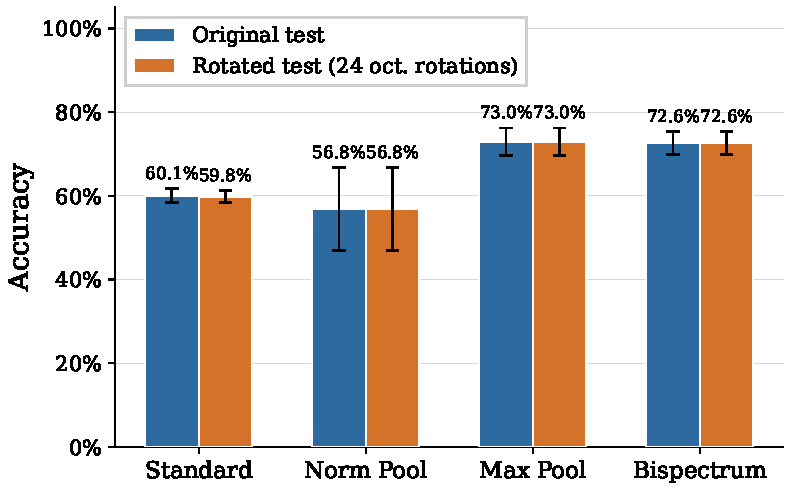
\includegraphics[width=0.75\linewidth]{experiments/organ3d/organ3d_analysis.pdf}
  \caption{OrganMNIST3D test accuracy on the original and octahedrally
    rotated test sets. Error bars show standard deviation over three
    seeds. All equivariant models achieve identical performance under
    rotation ($\sigma_{\mathrm{rot}} \approx 0$), while the
    augmentation-trained standard CNN degrades.}
  \label{fig:organ3d-rotation}
\end{figure}

\subsection{Wider channels}

To test whether the advantage of bispectral completeness persists at
higher capacity, we run max pool and bispectrum at channel widths
$(8, 16)$ and $(16, 32)$ with full training data.

\begin{table}[h]
  \caption{OrganMNIST3D accuracy at wider channel configurations
    (mean $\pm$ std over 3 seeds, full training data).}
  \label{tab:organ3d-wider}
  \centering
  \small
  \begin{tabular}{lrcc}
    \toprule
    Channels & Params & Max Pool & Bispectrum \\
    \midrule
    $(4, 8)$   & ${\sim}$375K / 463K  & $.730 \pm .033$ & $.726 \pm .027$ \\
    $(8, 16)$  & ${\sim}$1.5M / 1.7M  & $.743 \pm .015$ & $.745 \pm .006$ \\
    $(16, 32)$ & ${\sim}$6.0M / 6.3M  & $\mathbf{.785 \pm .032}$ & $.685 \pm .039$ \\
    \bottomrule
  \end{tabular}
\end{table}

At $(8, 16)$ the two methods are equivalent ($74.5 \pm 0.6\%$ bispectrum vs.\
$74.3 \pm 1.5\%$ max pool, both at ${\sim}1.5$--$1.7$M parameters). At $(16, 32)$ max
pool reaches $78.5 \pm 3.2\%$ while bispectrum drops to $68.5 \pm 3.9\%$---the 6.3M
parameter bispectrum model likely overfits the 971 training samples.
This suggests that the bispectrum's completeness advantage is most
pronounced in the data-limited rather than the parameter-limited
regime, consistent with the data efficiency findings in the main text.

\section{Experimental Details}
\label{app:exp}

\subsection{Hyperparameters}

Table~\ref{tab:hyperparams} summarises the training hyperparameters
for all three experimental settings.

\begin{table}[h]
  \caption{Training hyperparameters across experiments.}
  \label{tab:hyperparams}
  \centering
  \small
  \setlength{\tabcolsep}{4pt}
  \begin{tabular}{lccc}
    \toprule
    & PCam & OrganMNIST3D & Sph.\ MNIST \\
    \midrule
    Optimizer      & AdamW & AdamW & AdamW \\
    Learning rate  & $10^{-3}$ & $10^{-3}$ & $10^{-3}$ \\
    Weight decay   & $10^{-4}$ & $10^{-4}$ & $10^{-4}$ \\
    Batch size     & 64--256 & 16--64 & 256 \\
    Scheduler      & Cosine warm restarts & --- & --- \\
    Max epochs     & 50 & 100 & 50 \\
    Early stopping & Val AUC, pat.\ 10 & Val AUC, pat.\ 15 & Val ACC, pat.\ 10 \\
    Seeds          & 42, 123, 456$^\dagger$ & 42, 123, 456 & 42, 123, 456 \\
    Mixed precision & Yes & No & No \\
    \bottomrule
  \end{tabular}

  \vspace{0.3em}
  {\small $^\dagger$Pareto figure uses seed 42; matched-parameter table and data efficiency use seeds 42, 123, 456.}
\end{table}

\subsection{Hardware}

All experiments were run on a single NVIDIA H100 GPU (80\,GB).
Training wall-clock times range from ${\sim}$5 minutes (OrganMNIST3D,
971 samples) to ${\sim}$20 minutes (PCam, 26K samples at 10\% data).
Spherical MNIST bispectrum computation (forward pass through
\texttt{SO3onS2} at $\ell_{\max} = 15$) takes ${\sim}$0.3s per batch
of 64 on GPU.

\subsection{Data preprocessing}

\paragraph{PCam.}
PatchCamelyon~\citep{veeling2018rotation} consists of 327{,}680 RGB
patches of size $96 \times 96$ pixels extracted from whole-slide
images of lymph node sections~\citep{bejnordi2017camelyon}. We use
the standard train/val/test split. Images are loaded from HDF5 files
and normalised to $[0, 1]$. The standard (non-equivariant) baseline
uses random rotation and reflection augmentation during training; all
equivariant models are trained without augmentation.

\paragraph{OrganMNIST3D.}
OrganMNIST3D~\citep{medmnistv2} contains 1{,}742 abdominal CT organ
volumes of size $28 \times 28 \times 28$ voxels with 11 organ classes
(train/val/test = 971/161/610). Volumes are normalised to $[0, 1]$.
The standard baseline uses random octahedral augmentation (one of 24
rotations per sample); equivariant models are trained without
augmentation. Kernel rotations are implemented as exact voxel
permutations on the $3^3$ grid, avoiding interpolation artifacts.

\begin{table}[h]
  \caption{OrganMNIST3D (mean $\pm$ std, 3 seeds). Bispectral pooling
    matches max pool ($72.6\%$ vs.\ $73.0\%$), far exceeds norm pool
    ($56.8\%$), and delivers near-exact invariance
    ($\sigma_{\mathrm{rot}} \le 0.0005$).}
  \label{tab:organ3d-results}
  \centering
  \small
  \begin{tabular}{lrcccr}
    \toprule
    Model & Params & Test ACC & Test AUC & Rot ACC & $\sigma_{\mathrm{rot}}$ \\
    \midrule
    Standard 3D CNN          & 16K  & $.601 \pm .017$ & $.951 \pm .002$ & .598 & .0115 \\
    $O$-Equiv + Norm Pool    & 375K & $.568 \pm .099$ & $.940 \pm .021$ & .568 & .0000 \\
    $O$-Equiv + Max Pool     & 374K & $.730 \pm .033$ & $.972 \pm .005$ & .730 & .0000 \\
    $O$-Equiv + \texttt{OctaonOcta} Bispectrum   & 463K & $.726 \pm .027$ & $.972 \pm .004$ & .726 & .0005$^\dagger$ \\
    \bottomrule
  \end{tabular}

  \vspace{0.3em}
  {\small $^\dagger$Nonzero $\sigma_{\mathrm{rot}}$ due to floating-point precision in CG contractions, not a theoretical invariance failure.}
\end{table}


\paragraph{Spherical MNIST.}
MNIST digits are projected onto the sphere via stereographic
projection following \citet{cohen2018spherical} and sampled on a
$64 \times 128$ equiangular grid. The selective bispectrum is
computed at $\ell_{\max} = 15$, producing 384 complex invariant
coefficients. The model input is obtained by applying
$\operatorname{sign}(x)\log(1+|x|)$ separately to the real and
imaginary parts of each coefficient (a sign-preserving, per-channel
injective transform), giving 768 real features. These features are
fed to a 3-layer MLP: Linear(768, 256)--BN--ReLU--Linear(256,
128)--BN--ReLU--Linear(128, 10). The power spectrum MLP uses the
same structure with hidden=128: Linear(16, 128)--BN--ReLU--Linear(128,
64)--BN--ReLU--Linear(64, 10). The standard CNN has 4 convolutional
layers (16--32--64--64 channels) followed by adaptive average pooling
and a Linear(1024, 128)--ReLU--Linear(128, 10) classifier.

\subsection{Aggregation procedures}

\paragraph{PCam.}
The Pareto figure (Figure~\ref{fig:pcam-pareto}) uses a single seed
(42) across the full growth-rate sweep. The matched-parameter table
(Table~\ref{tab:pcam-results}) and data efficiency analysis use 3 seeds
(42, 123, 456) per configuration.

\paragraph{OrganMNIST3D.}
All results in Table~\ref{tab:organ3d-results} report mean $\pm$ std
over 3 seeds (42, 123, 456). Rotation robustness
($\sigma_{\mathrm{rot}}$) is the standard deviation of test accuracy
across all 24 octahedral rotations of the test set. The data
efficiency analysis (Figure~\ref{fig:data-efficiency} in the main text) uses 3 seeds per data
fraction.

\paragraph{Spherical MNIST.}
All results in Table~\ref{tab:smnist-results} report mean $\pm$ std
over 3 seeds (42, 123, 456). Rotation robustness
($\sigma_{\mathrm{rot}}$) is measured by applying 10 random $\SO(3)$
rotations to the entire test set and computing the standard deviation
of accuracy, yielding 30 measurements per model (10 rotations
$\times$ 3 seeds).

\subsection{Spherical MNIST: bispectrum reconstruction protocol}
\label{app:so3-recon}

This section gives the protocol behind
Figure~\ref{fig:so3-reconstruction} (Section~\ref{sec:so3-recon}).
The implementation lives in
\texttt{experiments/spherical\_mnist\_reconstruction/reconstruct.py}.

\paragraph{Setup.}
Spherical MNIST is rendered onto an equiangular $64{\times}128$
lat--lon grid using the same stereographic projection as the
classifier, then band-limited at $L = 12$ via a forward/inverse SHT
roundtrip (\texttt{torch\_harmonics.RealSHT}). For each digit we
draw a target rotation $R\in\SO(3)$ uniformly at random and form
$f := R\cdot f_0$. We compute the SO(3)-on-$S^2$ selective bispectrum
$\beta := \Phi_{\mathrm{sel}}(f)$.

\paragraph{Reconstruction.}
Starting from a Gaussian initialization $\hat f_0\sim\mathcal{N}(0, I)$
on the $64{\times}128$ grid, we optimize $\hat f$ with Adam
(initial LR $5\times 10^{-2}$, cosine annealing to $5\times 10^{-4}$,
$8000$ steps) to minimize the relative complex L2 loss
$\|\beta(\hat f) - \beta\|^2 / \|\beta\|^2$. After every step we
project $\hat f$ back to the band-limited subspace via $\mathrm{SHT}^{-1}\!\circ\mathrm{SHT}$ truncated at $L$ to suppress the
unconstrained null space. We run $4$ random restarts and keep the
$\hat f$ with the lowest bispectrum residual. Reconstruction
typically reaches $\|\beta(\hat f)-\beta\|/\|\beta\|\sim 10^{-3}$,
near the SHT-discretization invariance floor for this grid.

\paragraph{$\SO(3)$ alignment.}
The bispectrum is invariant on $\SO(3)$-orbits, so $\hat f$ lives
somewhere in the orbit of $f$ rather than at $f$ itself. We resolve
the orbit ambiguity by Procrustes-style fitting: we parameterize
$\hat R \in \SO(3)$ as a unit quaternion (auto-normalized) to avoid
gimbal lock, and minimize $\|\hat R\cdot\hat f - f\|^2$ with Adam
($12$ random restarts, $200$ steps each, cosine-annealed LR).
Rotations of the spherical image use bilinear interpolation in
lat--lon coordinates (\texttt{bispectrum.rotate\_spherical\_function}).

\paragraph{Numerical floor.}
On a $64{\times}128$ grid, two SHT roundtrips of two $\SO(3)$-rotated
copies of the same signal already differ by
$\|f' - f\|/\|f\|\approx 2\times 10^{-2}$ in image space due to
bilinear-interpolation discretization; this is the noise floor below
which alignment cannot improve. The aligned residuals reported in
Figure~\ref{fig:so3-reconstruction} ($0.1$--$0.3$) sit one to two
orders of magnitude above this floor and are dominated by gradient
descent local optima on the bispectrum reconstruction step, not by
missing information.

\subsection{Dataset licenses}

\begin{itemize}[nosep]
  \item \textbf{PCam}: CC0 1.0 Universal (public domain).
  \item \textbf{OrganMNIST3D}: CC BY 4.0.
  \item \textbf{Spherical MNIST}: derived from MNIST, which is
    publicly available for research use.
\end{itemize}

\section{API Example}
\label{app:api-example}

\begin{lstlisting}
import torch
from bispectrum import CnonCn, SO2onDisk, OctaonOcta

bsp = CnonCn(n=8, selective=True)
f = torch.randn(16, 8)
beta = bsp(f)
f_rec = bsp.invert(beta)
\end{lstlisting}

\end{document}